\documentclass[aspectratio=169]{beamer}

\usepackage{amsmath, amssymb, amsxtra, amsthm, amsfonts}
\usetheme{moloch}
\usecolortheme{beaver}
\setbeamertemplate{footline}
{
  \leavevmode%
  \hbox{%
    \begin{beamercolorbox}[wd=.5\paperwidth,ht=2.25ex,dp=1ex,center]{author in head/foot}%
      \usebeamerfont{author in head/foot}\insertsection
    \end{beamercolorbox}%
    \begin{beamercolorbox}[wd=.5\paperwidth,ht=2.25ex,dp=1ex,right]{date in head/foot}%
      \usebeamerfont{date in head/foot}\inserttitle\hspace*{2em}
      \insertframenumber{} / \inserttotalframenumber\hspace*{2ex}
    \end{beamercolorbox}}%
  \vskip0pt%
}
\makeatother

\usepackage[english]{babel}
\usefonttheme{serif}

\usepackage{mathtools}
\usepackage{graphicx}
\usepackage{bm}
\usepackage{color}
\usepackage[dvipsnames,table]{xcolor}
\usepackage{tikz}
\usepackage{stanli}
\usepackage{verbatim}
\usepackage{tikz}
\usetikzlibrary{shapes,calc,through,3d,patterns}
\usetikzlibrary{decorations.pathreplacing}
\usetikzlibrary{arrows.meta,calc,positioning}

\usepackage{pgfplots}
\usepackage{siunitx} % For formatting numbers
\usepackage{hyperref}
\hypersetup{colorlinks=true,linkcolor=darkred}
\usepackage{multicol}
\usepackage[absolute,overlay,]{textpos}
\usepackage{pgfplots}
\pgfplotsset{width=10cm,compat=1.9}
\usepackage{subcaption}
\usepackage{multirow}
\usepackage{bbding}
\usepackage{arydshln}
\usepackage{mathtools}
\usepackage{tcolorbox}
\usepackage{animate}

\textblockorigin{80mm}{45mm}


\newtheorem{thm}{Theorem}
\newtheorem{cor}[thm]{Corollary}
\newtheorem{prop}[thm]{Proposition}
\newtheorem{lem}[thm]{Lemma}
\theoremstyle{remark}
\newtheorem*{rem}{Remark}

%Block def
\definecolor{darkred}{rgb}{0.6,0,0}
\setbeamertemplate{blocks}[rounded][shadow=false]
\setbeamercolor{block title}{bg=darkred!15,fg=black}
\setbeamercolor{block body}{bg=darkred!5,fg=black}

\setbeamercolor{itemize item}{fg=darkred}
\setbeamercolor{itemize subitem}{fg=darkred}
\setbeamercolor{itemize subsubitem}{fg=darkred}
\setbeamercolor{enumerate item}{fg=darkred}
\setbeamercolor{button}{bg=gray!30,fg=darkred}

\setbeamertemplate{itemize item}[square]
\setbeamertemplate{itemize subitem}[circle]
\setbeamertemplate{itemize subsubitem}[triangle]
\setbeamertemplate{enumerate items}[circle]
\setbeamercolor{item projected}{bg=darkred}

\newcommand{\bolddelta}{\boldsymbol\delta}
\newcommand{\boldxi}{\boldsymbol\xi}
\DeclareMathOperator*{\A}{\text{\raisebox{-0.2cm}{\Huge A}}}




\title{Dynamic analysis of trusses}
\subtitle{Special structural elements}
\author{ME473 Dynamic finite element analysis of structures}
\institute{Stefano Burzio}
\date{2025}

\begin{document}
\usenavigationsymbolstemplate{}
{\setbeamertemplate{footline}{}

  \frame{\titlepage
    \begin{tikzpicture}[overlay, remember picture]
      \node[anchor=north east, xshift=-.9cm] at (current page.north east) {
\includegraphics[width=2cm]{../images/epfl_logo.png}};
      \node[anchor=south east, xshift=-.87cm, yshift=.05cm] at (current page.south east)  {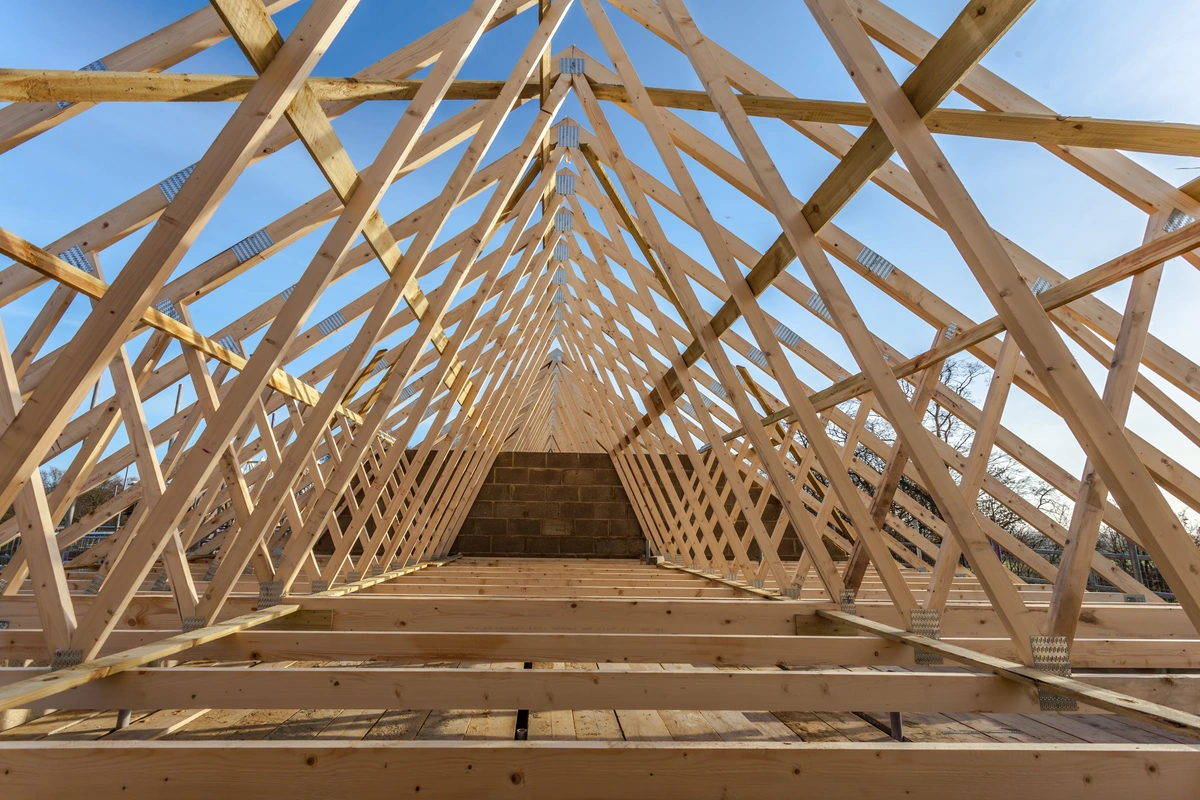
\includegraphics[width=5cm]{../images/roofTrussStructure.png}};
    \end{tikzpicture}
  }


  \begin{frame}{Where do we stand?}
    \begin{center}
      \begin{tabular}{|c|l|l|l|}
        \hline
        \rowcolor{darkred!20}\textbf{Week} & \textbf{Module}                          & \textbf{Lecture topic}             & \textbf{Mini-projects} \\
        \hline
        1                                  & \multirow{5}{7em}{Linear elastodynamics} & Strong and weak forms              &                        \\ \cline{1-1} \cline{3-4}
        2                                  &                                          & Galerkin and FE methods            &                        \\ \cline{1-1} \cline{3-4}
        3                                  &                                          & Systematisation of the procedure   & Groups formation       \\ \cline{1-1} \cline{3-4}
        4                                  &                                          & 3d elements, numerical integration & Project 1 statement    \\
        \cline{1-1} \cline{3-4}
        \hline
        5                                  & Special                                  & Bars and trusses                   &                        \\
                                           & structural                               &                                    &                        \\
                                           & elements                                 &                                    &                        \\
        \hline
      \end{tabular}
    \end{center}
    \vspace{1cm}
  \end{frame}

  \begin{frame}
    \textbf{\large Summary}
    \begin{itemize}
      \item Recap weeks 1 to 4
      \item Eigenvalues and eigenvectors errors bounds
      \item Trusses in 2d
            \begin{itemize}
              \item Illustrative example of a 2d truss structure
              \item Matlab example of a 2d truss in free vibrations
            \end{itemize}
      \item Trusses in 3d
            \begin{itemize}
              \item Matlab example of a 3d truss in free vibrations
              \item Ansys example of a transient analysis of a Basketball hoop frame
            \end{itemize}
    \end{itemize}
    \vspace{.5cm}

    \textbf{\large Recommended readings}
    \begin{enumerate}
      \item Logan, A first course in the finite element method, 6th ed.
            (chap. 3)
      \item Paz and Leigh, Structural dynamics, 6th ed. (chap. 14)
      \item Ferreira and Fantuzzi, MATLAB Codes for Finite Element Analysis, 2nd ed. (chap. 4 and 5)
    \end{enumerate}
  \end{frame}
}

\section{\emph{Brief} recap of weeks 1 to 4 \\ FEM for elastodynamics of solids}
 {\setbeamercolor{background canvas}{bg=darkred!5}
  \setbeamercolor{block body}{bg=darkred!5,fg=black}

  \begin{frame}{Statement of the linear elastodynamics problem}
    \begin{columns}[T]
      \begin{column}{.8\textwidth}
        \begin{itemize}
          \item \textbf{Object:} \\ A solid $\Omega\subset\mathbb R^{3}$ with known material properties: $\mathbf C$ and $\rho$.
                \vspace{0.3cm}
          \item \textbf{Main features:}
                \begin{itemize}
                  \item Acting loads on the body: $\mathbf f$.
                        \vspace{0.1cm}
                  \item Boundary $\Gamma=\Gamma_{u}\cup\Gamma_{\sigma}$ (the surface enclosing the solid).
                        \vspace{0.1cm}
                  \item Boundary conditions: prescribed displacements $\mathbf{\hat u}$ on $\Gamma_{u}$ and/or loads $\mathbf{\hat f}$ on $\Gamma_{\sigma}$.
                        \vspace{0.1cm}
                  \item Initial displacement $\mathbf u_0$ and velocity $\mathbf v_0$ at $t=0$.
                \end{itemize}
        \end{itemize}
      \end{column}
      \begin{column}{.3\textwidth}
        \begin{center}
          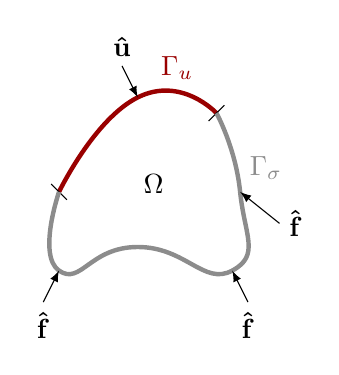
\begin{tikzpicture}
            % Label the region Omega	
            \node at (2.2,2.1) {$\Omega$};
            % Label the boundary Gamma
            \draw[ultra thick, darkred] plot [smooth, tension=1] coordinates {(1,2) (2,3.2) (3,3)};
            \node[darkred, above] at (2.5,3.3) {$\Gamma_u$};
            \draw[thin] (3+0.1,3+0.1) --(3-0.1,3-0.1);
            \draw[thin] (1+0.1,2-0.1) --(1-0.1,2+0.1);
            \draw[latex-]  (2,3.2) --  (2-0.2,3.2+0.4) node[above] {$\mathbf{\hat u}$};
            % Draw part of the boundary Gamma_sigma
            \draw[ultra thick, gray!90] plot [smooth, tension=1] coordinates {(3,3) (3.3,2) (3.2,1) (2,1.3) (1,1) (1,2)};
            \node[gray!90, right] at (3.3,2.3) {$\Gamma_\sigma$};
            \draw[latex-]  (1,1) --  (1-0.2,1-0.4) node[below] {$\mathbf{\hat f}$};;
            \draw[latex-]  (3.2,1) --  (3.2+0.2,1-0.4) node[below] {$\mathbf{\hat f}$};
            \draw[latex-]  (3.3,2) --  (3.3+0.5,2-0.4) node[right] {$\mathbf{\hat f}$};
          \end{tikzpicture}
        \end{center}
      \end{column}
    \end{columns}
  \end{frame}

  \begin{frame}{Strong and semi-discrete weak forms of elastodynamics}
    \vspace{-0.5cm}
    \begin{center}
      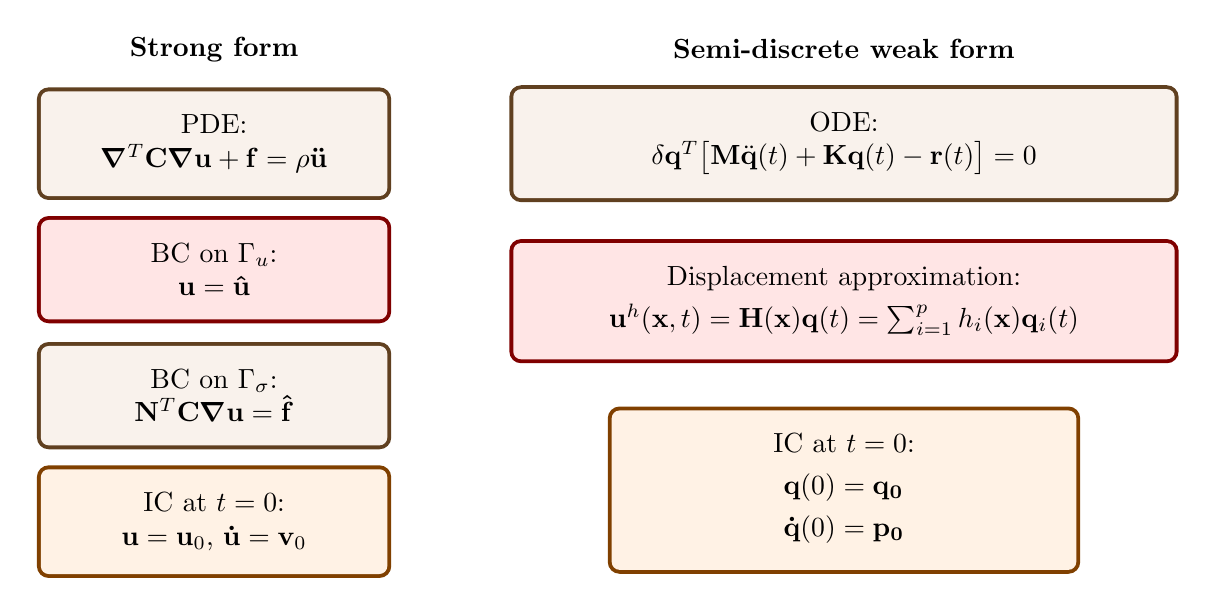
\begin{tikzpicture}[scale=0.8]
        \node (sf) at (-2,6.5) {
          \centering \textbf{Strong form}
        };
        \node (wf) at (8,6.5) {
          \centering \textbf{Semi-discrete weak form}
        };
        \node (pde) at (-2,5) {
          \begin{tcolorbox}[colframe=brown!50!black, colback=brown!10, coltitle=black, rounded corners, width=4.5cm]
            \centering PDE: \\ $\boldsymbol\nabla^T\mathbf C\boldsymbol\nabla \mathbf u+\mathbf f=\rho\mathbf{\ddot{u}}$
          \end{tcolorbox}
        };
        \node (bc1) at (-2,3) {
          \begin{tcolorbox}[colframe=red!50!black, colback=red!10, coltitle=black, rounded corners,width=4.5cm]
            \centering BC on $\Gamma_u$: \\ $\mathbf u=\mathbf{\hat u}$
          \end{tcolorbox}
        };
        \node (bc2) at (-2,1) {
          \begin{tcolorbox}[colframe=brown!50!black, colback=brown!10, coltitle=black, rounded corners,width=4.5cm]
            \centering BC on $\Gamma_\sigma$: \\ $\mathbf N^T\mathbf  C\boldsymbol\nabla\mathbf  u=\mathbf{\hat f}$
          \end{tcolorbox}
        };

        \node (ic1) at (-2,-1) {
          \begin{tcolorbox}[colframe=orange!50!black, colback=orange!10, coltitle=black, rounded corners,width=4.5cm]
            \centering IC at $t=0$: \\ $\mathbf{u}=\mathbf u_0$, $\mathbf{\dot u}=\mathbf v_0$
          \end{tcolorbox}
        };
        \node (inteq) at (8,5) {
          \begin{tcolorbox}[colframe=brown!50!black, colback=brown!10, coltitle=black, rounded corners, width=8.5cm]
            \centering ODE: \\  $\delta\mathbf q^{T}\big[\mathbf M\ddot{\mathbf q}(t)+\mathbf K\mathbf q(t)-\mathbf r(t)\big]=0$
          \end{tcolorbox}
        };
        \node (funcsp) at (8,2.5) {
          \begin{tcolorbox}[colframe=red!50!black, colback=red!10, coltitle=black, rounded corners,width=8.5cm]
            \centering Displacement approximation: \\[3pt]      $\mathbf u^{h}(\mathbf x,t)      =\mathbf H(\mathbf x)\mathbf q(t) = \sum_{i=1}^{p}h_{i}(\mathbf x)\mathbf q_{i}(t) $
          \end{tcolorbox}
        };
        \node (ic2) at (8,-0.5) {
          \begin{tcolorbox}[colframe=orange!50!black, colback=orange!10, coltitle=black, rounded corners,width=6cm]
            \centering IC at $t=0$: \\ \vspace{0.2cm} $\begin{aligned}
                 & \mathbf{q}(0)=\mathbf{q_{0}}      \\
                 & \mathbf{\dot q}(0)=\mathbf{p_{0}}
              \end{aligned}$
          \end{tcolorbox}
        };
      \end{tikzpicture}
    \end{center}
  \end{frame}

  \begin{frame}{Displacements approximation in finte element method}
    \vspace{-1cm}
    \begin{columns}[T]
      \begin{column}{.4\textwidth}
        \begin{center}
          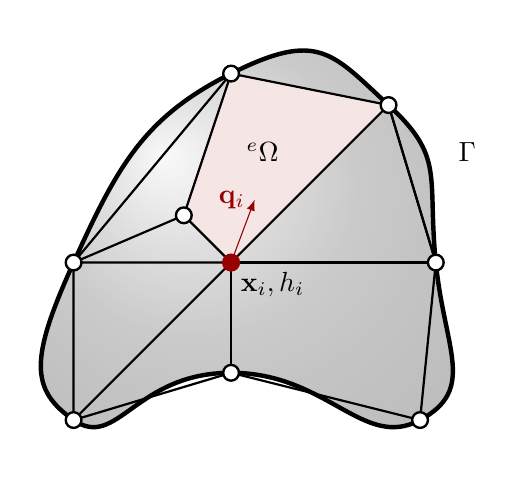
\begin{tikzpicture}[scale=2]
            %\draw[step=1.0,black,thin] (0,0) grid (4,4);
            % Draw the potato-like shape
            \shade [ball color= gray!90!black, opacity=.3] plot [thick,smooth cycle, tension=1] coordinates  {(1,2) (2,3.2) (3,3) (3.3,2) (3.2,1) (2,1.3) (1,1)};
            \draw[ultra thick] plot [thick,smooth cycle, tension=1] coordinates {(1,2) (2,3.2) (3,3) (3.3,2) (3.2,1) (2,1.3) (1,1)};
            \draw[fill=darkred!30,thick,darkred!10] (2,2) -- (3,3) -- (2,3.2) -- (1.7,2.3) -- cycle;
            \node[below right] at (2,2) {$\mathbf x_i, h_i$};
            \draw[-latex,darkred] (2,2) -- (2.15,2.4) node[darkred, left]{$\mathbf q_i$};
            % Label the region Omega	
            \node at (2.2,2.7) {${}^e\Omega$};
            % Label the boundary Gamma
            \node at (3.5,2.7) {$\Gamma$};
            \draw[thick] (1,2) -- (2,3.2) -- (3,3) -- (3.3,2) -- (3.2,1) -- (2,1.3) -- (1,1) -- cycle;
            \draw[thick] (1,2) -- (2,2) -- (3,3) -- (3.3,2);
            \draw[thick] (2,1.3) -- (2,2) -- (3.3,2);
            \draw[thick] (1,1) -- (2,2) -- (1.7,2.3) -- (2,3.2);
            \draw[thick] (1.7,2.3) -- (1,2);
            \node[darkred,draw,shape=circle,fill=darkred,minimum size=2mm,line width=0.3mm,inner sep=0] at (2,2) {};
            \node[draw,shape=circle,fill=white,minimum size=2mm,line width=0.3mm,inner sep=0] at (1,1) {};
            \node[draw,shape=circle,fill=white,minimum size=2mm,line width=0.3mm,inner sep=0] at (1,2) {};
            \node[draw,shape=circle,fill=white,minimum size=2mm,line width=0.3mm,inner sep=0] at (2,1.3) {};
            \node[draw,shape=circle,fill=white,minimum size=2mm,line width=0.3mm,inner sep=0] at (2,3.2) {};
            \node[draw,shape=circle,fill=white,minimum size=2mm,line width=0.3mm,inner sep=0] at (1.7,2.3) {};
            \node[draw,shape=circle,fill=white,minimum size=2mm,line width=0.3mm,inner sep=0] at (3,3) {};
            \node[draw,shape=circle,fill=white,minimum size=2mm,line width=0.3mm,inner sep=0] at (3.2,1) {};
            \node[draw,shape=circle,fill=white,minimum size=2mm,line width=0.3mm,inner sep=0] at (3.3,2) {};
          \end{tikzpicture}
        \end{center}
      \end{column}
      \begin{column}{.6\textwidth}
        \begin{block}{}
          \begin{itemize}
            \item \textbf{Stiffness matrix}:
                  $$\mathbf K=\int_\Omega \mathbf B^T\mathbf C\mathbf B \, d\Omega$$
                  where $\mathbf B=\nabla \mathbf H$.
            \item \textbf{Mass matrix}:
                  $$\mathbf M=\int_\Omega \rho\, \mathbf H^T\mathbf H \, d\Omega.$$
            \item \textbf{Applied forces vector}:
                  $$\mathbf r(t)=\int_{\Gamma_\sigma} \mathbf H^{T}\mathbf{\hat f} \, d\Gamma+\int_{\Omega} \mathbf H^{T}\mathbf f\, d\Omega.$$
          \end{itemize}
        \end{block}
      \end{column}
    \end{columns}
  \end{frame}


  \begin{frame}{Types of analysis}
    \begin{columns}[T,onlytextwidth]
      % ============================================================
      % STATIC
      % ============================================================
      \begin{column}{0.31\textwidth}
        \begin{block}{Static analysis}
          \centering
          \small
          \emph{Constant loads}

          \vspace{0.25cm}

          Determines the structural deformation
          $\mathbf q$ due to constant loads.
        \end{block}
      \end{column}

      % ============================================================
      % MODAL
      % ============================================================
      \begin{column}{0.31\textwidth}
        \begin{block}{Modal analysis}
          \centering
          \small
          \emph{Natural frequencies}

          \vspace{0.25cm}

          Studies the intrinsic dynamic properties of the structure.
        \end{block}
      \end{column}

      % ============================================================
      % TRANSIENT
      % ============================================================
      \begin{column}{0.31\textwidth}

        \begin{block}{Transient analysis}
          \centering
          \small
          \emph{Time-dependent loads}

          \vspace{0.25cm}

          Determines the structural response
          $\mathbf q(t)$ to time-dependent excitations
          $\mathbf r(t)$.
        \end{block}
      \end{column}
    \end{columns}

    \vspace{-0.5cm}

    \begin{columns}[T,onlytextwidth]
      % ============================================================
      % STATIC
      % ============================================================
      \begin{column}{0.31\textwidth}
        \begin{block}{}
          \centering
          \small
          \[
            \mathbf K\mathbf q=\mathbf r
          \]
          \vspace{-0.45cm}
          \footnotesize
          \begin{itemize}
            \item No inertia effects
            \item No time dependence
            \item Equilibrium between internal and external forces
          \end{itemize}
        \end{block}
      \end{column}

      % ============================================================
      % MODAL
      % ============================================================
      \begin{column}{0.31\textwidth}
        \begin{block}{}
          \centering
          \small
          \[
            \mathbf M\ddot{\mathbf q}(t)
            +
            \mathbf K\mathbf q(t)
            =
            \mathbf 0
          \]
          \vspace{-0.45cm}
          \footnotesize
          \begin{itemize}
            \item No external excitation
            \item Resonance when excitation frequency $\approx$ natural frequency
          \end{itemize}
        \end{block}
      \end{column}

      % ============================================================
      % TRANSIENT
      % ============================================================
      \begin{column}{0.31\textwidth}

        \begin{block}{}
          \centering
          \small
          \[
            \mathbf M\ddot{\mathbf q}(t)
            +
            \mathbf K\mathbf q(t)
            =
            \mathbf r(t)
          \]
          \vspace{-0.45cm}
          \footnotesize
          \begin{itemize}
            \item Inertia effects included
            \item Response evolves in time
            \item Used for impacts, vibrations and dynamic loading
          \end{itemize}
        \end{block}
      \end{column}
    \end{columns}
  \end{frame}
 }

\section{Eigenvalues and eigenvectors errors bounds}

\begin{frame}{A priori error estimates for eigenvalues and eigenvectors}
  Using principles from Rayleigh and Courant-Fischer, asymptotic error estimates can be established for eigenvalues and eigenvectors for conformal elements.
  \begin{tcolorbox}[colback=darkred!10,colframe=darkred!40!black]
    \vspace{-0.5cm}
    \begin{align*}
      \lambda_i \leq \lambda_i^h                              & \leq \lambda_i + c\, h^{2(m-k+1)}\, \lambda_i^{m+1}    \\
      \| \boldsymbol{\phi}_i^h - \boldsymbol{\phi}_i \|_{L^2} & \leq c\, h^{\min(m+1, 2(m-k+1))}\, \lambda_i^{(m+1)/2}
    \end{align*}
  \end{tcolorbox}
  \begin{itemize}
    \setlength\itemsep{0.5em}
    \item \( \lambda_i^h \) are the \emph{approximated} eigenvalues and \(\boldsymbol \phi_i^h \) the corresponding eigenvectors,
    \item  \( \lambda_i \) are the \emph{exact} eigenvalues and \(\boldsymbol\phi_i \) the corresponding eigenvectors,
    \item \( h \) represents the characteristic mesh size,
    \item \( m \) is the degree of the highest complete polynomial used,
    \item \( k \) is the the highest derivative order appearing in the weak form,
    \item \( c \) is a constant independent of \( h \).
  \end{itemize}
\end{frame}

\begin{frame}{A priori error estimates for frequencies}
  \vspace{-0.3cm}
  From the relationship between eigenvalues and frequencies,  $\omega_i^h=\sqrt{\lambda_i^h}$, we deduce the bound on the approximate frequencies.
  \begin{tcolorbox}[colback=darkred!10,colframe=darkred!40!black]
    $$ \omega_i \leq \omega_i^h \leq \omega_i + c\, h^{2(m-k+1)}\, \omega_i^{2m+1}$$
  \end{tcolorbox}
  \begin{itemize}
    \setlength\itemsep{0.5em}
    \item {Approximate frequencies $\omega_i^h$ always overestimate the exact frequencies $\omega_i$.}
    \item {The quality of approximated frequencies degrades for higher frequencies.}
    \item The convergence rates for eigenvectors and frequencies are both of order \( h^{2m} \) for weak forms with \( k=1 \) (e.g. elastodynamics).
  \end{itemize}
\end{frame}

\section{Structural 1d elements : general ideas}

\begin{frame}
  \frametitle{\textbf{Example:} analysis of the forth bridge}
  \begin{center}
    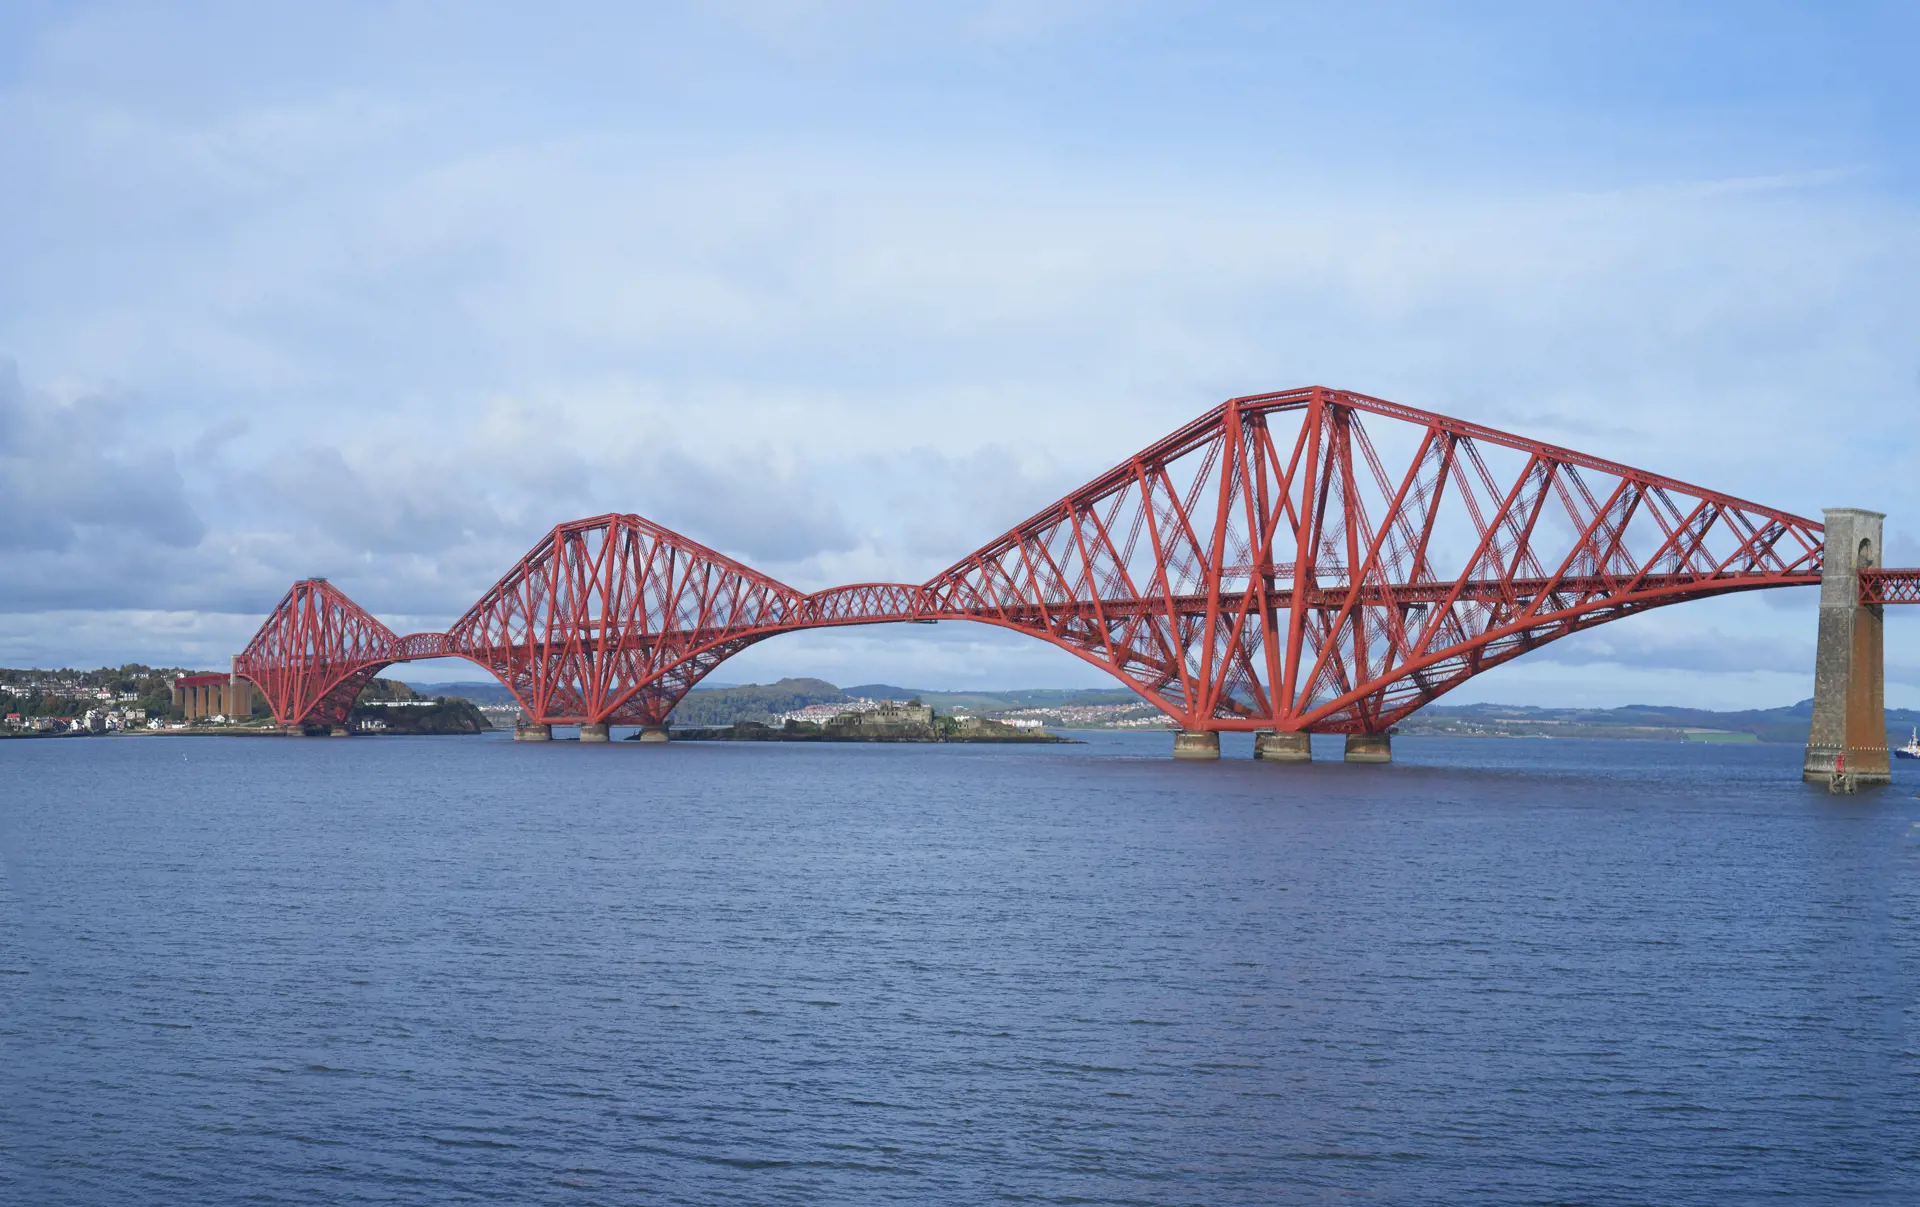
\includegraphics[height=3cm]{../images/fortrailbridge}

    {\footnotesize (Credit:
      \hyperlink{https://www.theforthbridges.org/about-the-forth-bridges/forth-bridge/}{theforthbridges.org})}

    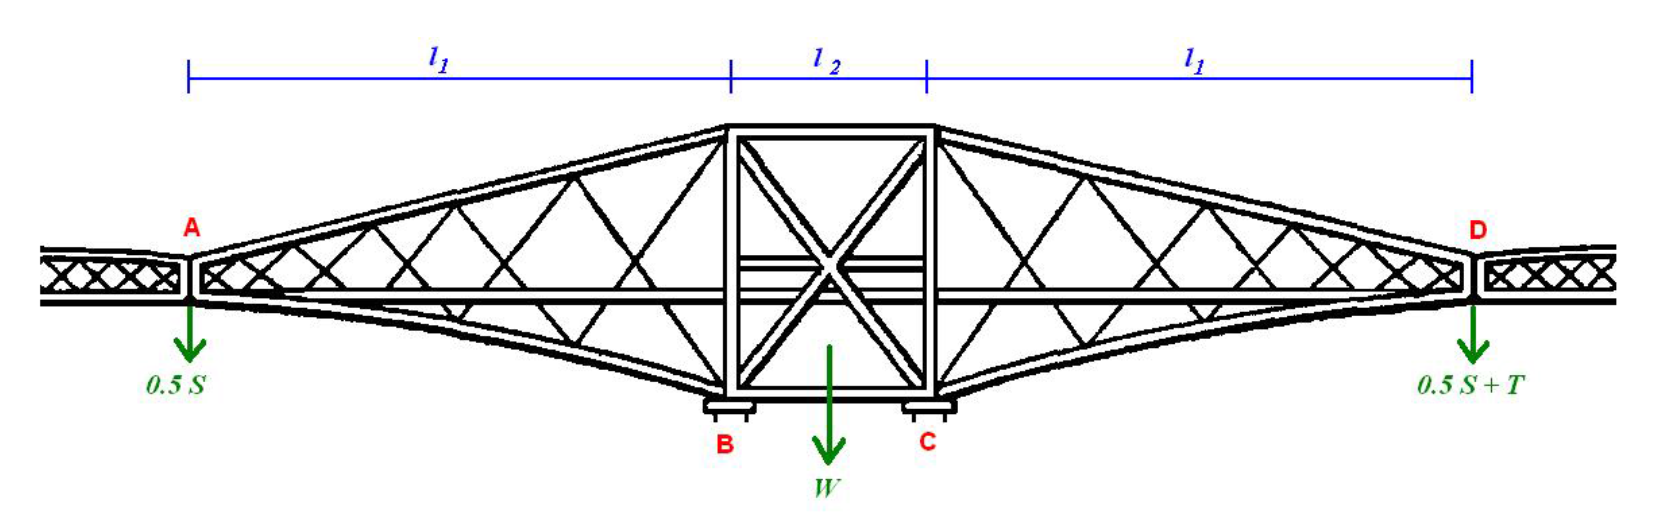
\includegraphics[height=3cm]{../images/fortrailbridgeScheme}

    {\footnotesize (Credit:
      \hyperlink{https://ethz.ch/content/dam/ethz/special-interest/baug/ibk/structural-mechanics-dam/education/femI/2024/Lecture_1_EC_2024.pdf}{Chatzi and Egger})}
  \end{center}
\end{frame}

\begin{frame}
  \frametitle{Abstract model}
  \begin{center}
    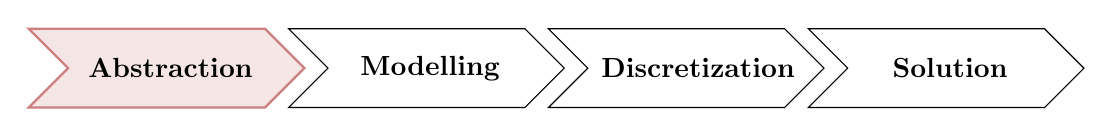
\begin{tikzpicture}
      % First arrow
      \draw[thick,fill=darkred!10,draw=darkred!50] (-3.3,0) -- (-0.3,0) -- (0.2,0.5) -- (-0.3,1) -- (-3.3,1) -- (-2.8,0.5) -- cycle;
      \node at (-1.5,0.5) {\textbf{Abstraction}};
      % Second arrow
      \draw[fill=white] (0,0) -- (3,0) -- (3.5,0.5) -- (3,1) -- (0,1) -- (0.5,0.5) -- cycle;
      \node at (1.8,0.5) {\textbf{Modelling}};
      % Third arrow
      \draw[fill=white] (3.3,0) -- (6.3,0) -- (6.8,0.5) -- (6.3,1) -- (3.3,1) -- (3.8,0.5) -- cycle;
      \node at (5.2,0.5) {\textbf{Discretization}};
      % Fourth arrow
      \draw[fill=white] (6.6,0) -- (9.6,0) -- (10.1,0.5) -- (9.6,1) -- (6.6,1) -- (7.1,0.5) -- cycle;
      \node at (8.4,0.5) {\textbf{Solution}};
    \end{tikzpicture}
  \end{center}
  \begin{columns}
    \begin{column}{0.5\textwidth}
      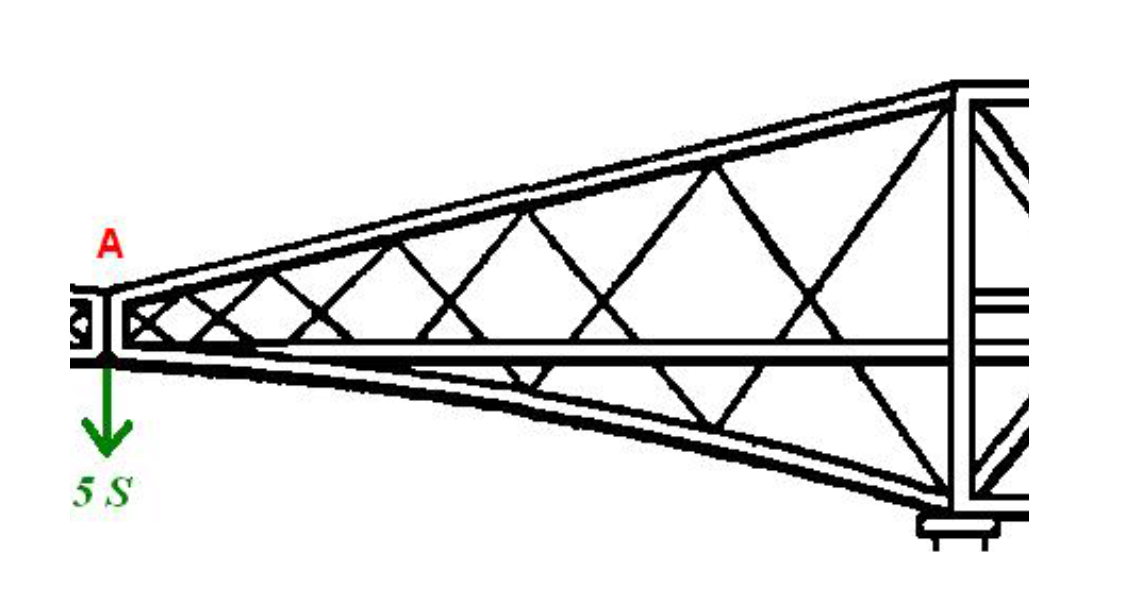
\includegraphics[height=4cm]{../images/fortrailbridgePartScheme}
      {\footnotesize (Credit:
        \hyperlink{https://ethz.ch/content/dam/ethz/special-interest/baug/ibk/structural-mechanics-dam/education/femI/2024/Lecture_1_EC_2024.pdf}{Chatzi and Egger})}
    \end{column}
    \begin{column}{0.5\textwidth}
      \textbf{Conceptual framework:} develop a simplified idealisation of the structure, or part of the structure, representing the geometry and loads.
    \end{column}
  \end{columns}
\end{frame}

\begin{frame}
  \frametitle{Mathematical model}
  \begin{center}
    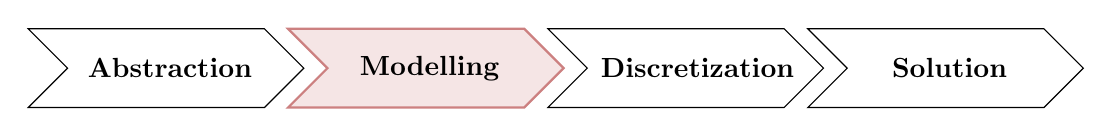
\begin{tikzpicture}
      % First arrow
      \draw[fill=white](-3.3,0) -- (-0.3,0) -- (0.2,0.5) -- (-0.3,1) -- (-3.3,1) -- (-2.8,0.5) -- cycle;
      \node at (-1.5,0.5) {\textbf{Abstraction}};
      % Second arrow
      \draw[thick,fill=darkred!10,draw=darkred!50]  (0,0) -- (3,0) -- (3.5,0.5) -- (3,1) -- (0,1) -- (0.5,0.5) -- cycle;
      \node at (1.8,0.5) {\textbf{Modelling}};
      % Third arrow
      \draw[fill=white] (3.3,0) -- (6.3,0) -- (6.8,0.5) -- (6.3,1) -- (3.3,1) -- (3.8,0.5) -- cycle;
      \node at (5.2,0.5) {\textbf{Discretization}};
      % Fourth arrow
      \draw[fill=white] (6.6,0) -- (9.6,0) -- (10.1,0.5) -- (9.6,1) -- (6.6,1) -- (7.1,0.5) -- cycle;
      \node at (8.4,0.5) {\textbf{Solution}};
    \end{tikzpicture}
  \end{center}
  \begin{columns}
    \begin{column}{0.5\textwidth}
      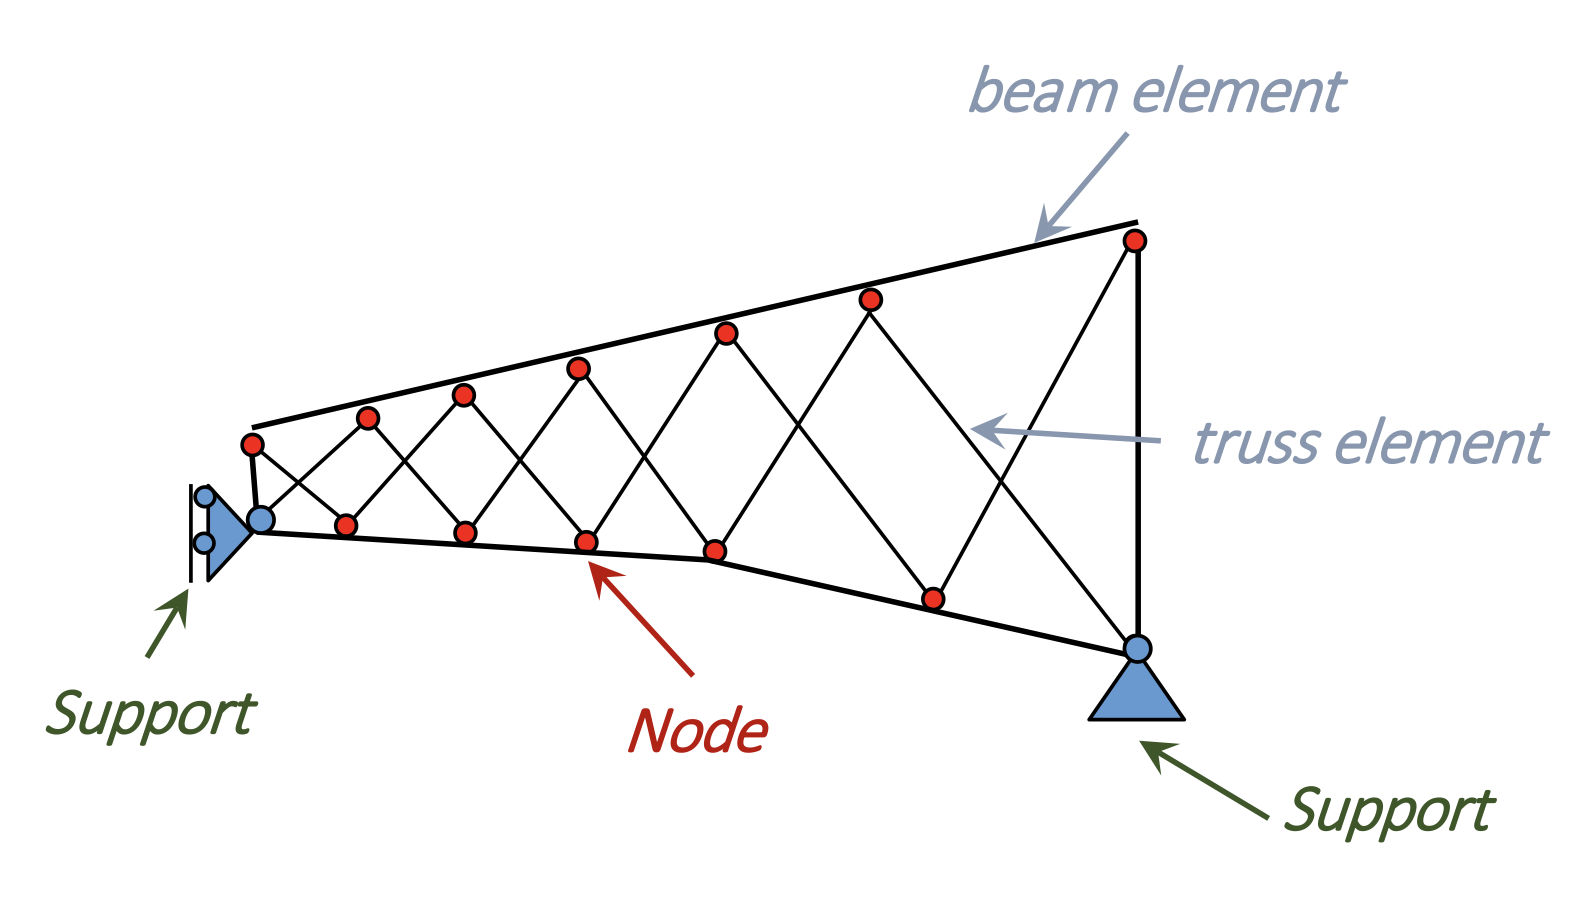
\includegraphics[height=4cm]{../images/fortrailbridgeSchemeMath}
      {\footnotesize (Credit:
        \hyperlink{https://ethz.ch/content/dam/ethz/special-interest/baug/ibk/structural-mechanics-dam/education/femI/2024/Lecture_1_EC_2024.pdf}{Chatzi and Egger})}
    \end{column}
    \begin{column}{0.5\textwidth}
      Connect the structure to a known theoretical model capable of describing its functioning with sufficient accuracy.
      \vspace{0.3cm}

      \textbf{Assumption:} decompose the system into 1D components, such as trusses and beams.
    \end{column}
  \end{columns}
\end{frame}

\begin{frame}
  \frametitle{Discrete model}
  \begin{center}
    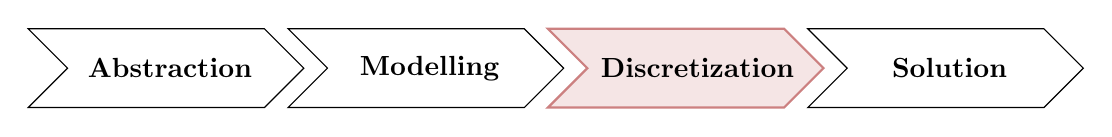
\begin{tikzpicture}
      % First arrow
      \draw[fill=white] (-3.3,0) -- (-0.3,0) -- (0.2,0.5) -- (-0.3,1) -- (-3.3,1) -- (-2.8,0.5) -- cycle;
      \node at (-1.5,0.5) {\textbf{Abstraction}};
      % Second arrow
      \draw[fill=white] (0,0) -- (3,0) -- (3.5,0.5) -- (3,1) -- (0,1) -- (0.5,0.5) -- cycle;
      \node at (1.8,0.5) {\textbf{Modelling}};
      % Third arrow
      \draw[thick,fill=darkred!10,draw=darkred!50] (3.3,0) -- (6.3,0) -- (6.8,0.5) -- (6.3,1) -- (3.3,1) -- (3.8,0.5) -- cycle;
      \node at (5.2,0.5) {\textbf{Discretization}};
      % Fourth arrow
      \draw[fill=white] (6.6,0) -- (9.6,0) -- (10.1,0.5) -- (9.6,1) -- (6.6,1) -- (7.1,0.5) -- cycle;
      \node at (8.4,0.5) {\textbf{Solution}};
    \end{tikzpicture}
  \end{center}
  \begin{columns}
    \begin{column}{0.5\textwidth}
      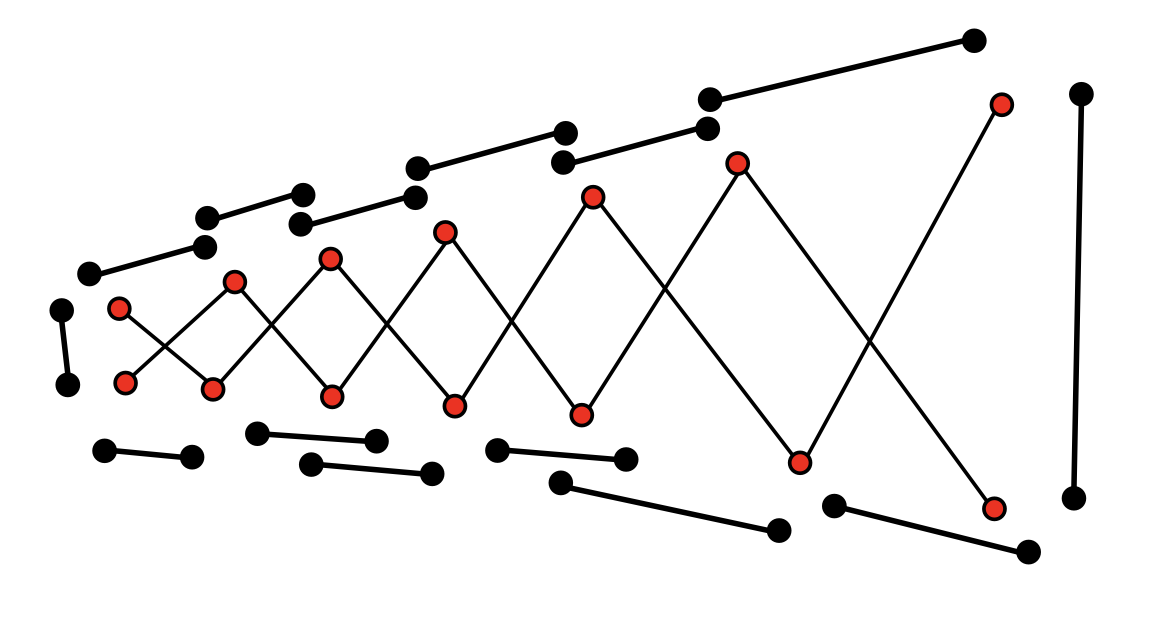
\includegraphics[height=4cm]{../images/fortrailbridgeSchemeDisassembled}
      {\footnotesize (Credit:
        \hyperlink{https://ethz.ch/content/dam/ethz/special-interest/baug/ibk/structural-mechanics-dam/education/femI/2024/Lecture_1_EC_2024.pdf}{Chatzi and Egger})}
    \end{column}
    \begin{column}{0.5\textwidth}
      \vspace{-0.8cm}

      \textbf{Direct stiffness method framework:} the continuum is disassembled using a mesh of finite elements that are connected at nodes located on the
      element boundaries.
    \end{column}
  \end{columns}
\end{frame}

\begin{frame}
  \frametitle{Deformed model}
  \begin{center}
    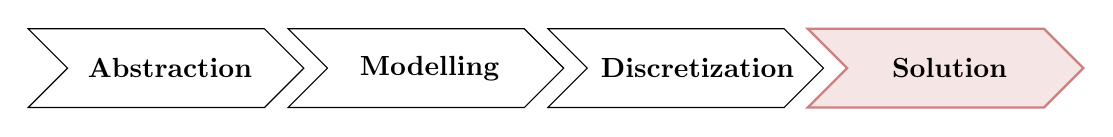
\begin{tikzpicture}
      % First arrow
      \draw[fill=white] (-3.3,0) -- (-0.3,0) -- (0.2,0.5) -- (-0.3,1) -- (-3.3,1) -- (-2.8,0.5) -- cycle;
      \node at (-1.5,0.5) {\textbf{Abstraction}};
      % Second arrow
      \draw[fill=white] (0,0) -- (3,0) -- (3.5,0.5) -- (3,1) -- (0,1) -- (0.5,0.5) -- cycle;
      \node at (1.8,0.5) {\textbf{Modelling}};
      % Third arrow
      \draw[fill=white] (3.3,0) -- (6.3,0) -- (6.8,0.5) -- (6.3,1) -- (3.3,1) -- (3.8,0.5) -- cycle;
      \node at (5.2,0.5) {\textbf{Discretization}};
      % Fourth arrow
      \draw[thick,fill=darkred!10,draw=darkred!50] (6.6,0) -- (9.6,0) -- (10.1,0.5) -- (9.6,1) -- (6.6,1) -- (7.1,0.5) -- cycle;
      \node at (8.4,0.5) {\textbf{Solution}};
    \end{tikzpicture}
  \end{center}
  \begin{columns}
    \begin{column}{0.5\textwidth}
      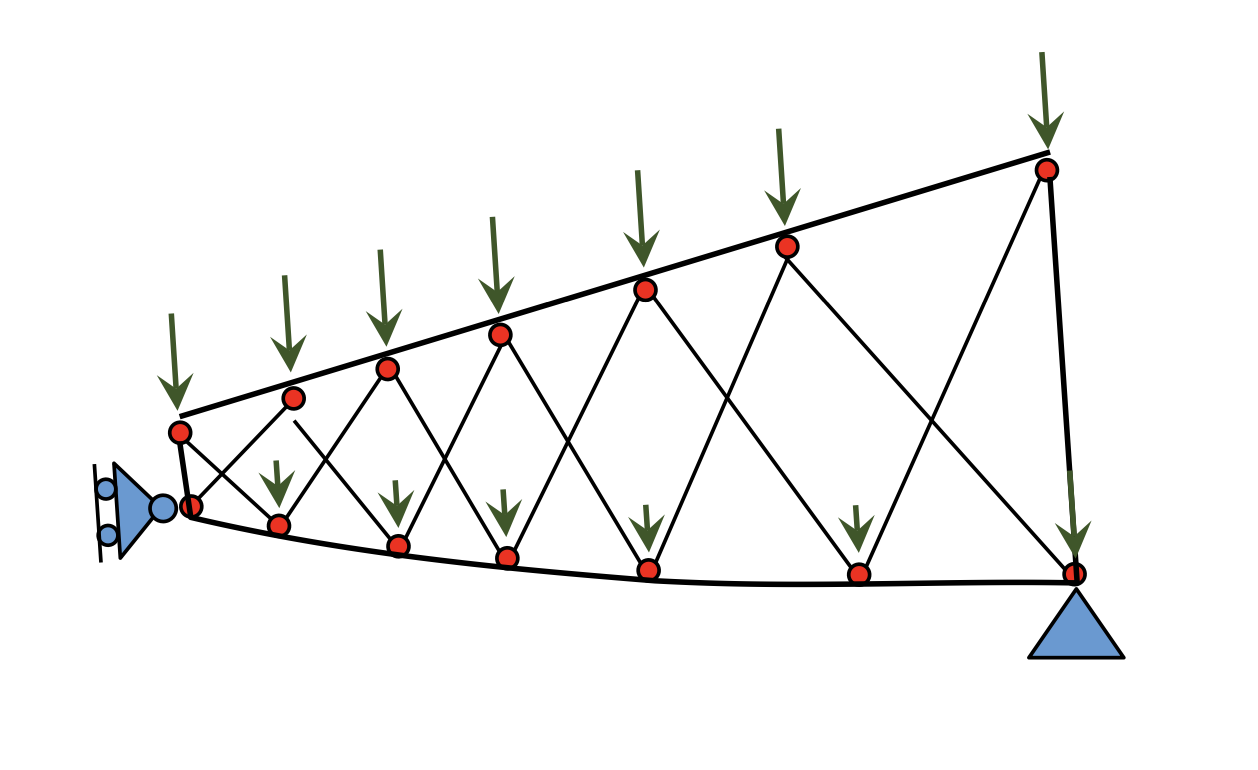
\includegraphics[height=4cm]{../images/fortrailbridgeSchemeSolution}
      {\footnotesize (Credit:
        \hyperlink{https://ethz.ch/content/dam/ethz/special-interest/baug/ibk/structural-mechanics-dam/education/femI/2024/Lecture_1_EC_2024.pdf}{Chatzi and Egger})}
    \end{column}
    \begin{column}{0.5\textwidth}
      \vspace{-0.8cm}

      Solve for the structure degrees of freedom:
      \begin{itemize}
        \item \textbf{assembly} of element quantities and application of boundary conditions,
        \item \textbf{post-processing:} computation of strains, stresses, reaction forces, and moments.
      \end{itemize}
    \end{column}
  \end{columns}
\end{frame}

\section{Trusses in 2d}

\begin{frame}{What is a truss structure?}
  \begin{columns}[T,onlytextwidth]
    \begin{column}{0.56\textwidth}
      \textbf{Plane truss}
      \small
      \begin{itemize}
        \item A structure composed of oriented bar (rod) elements that lie in a common plane and are connected by frictionless pins.
        \item Loads act only in the common plane and are applied at the nodes or joints.
        \item Trusses are commonly used in steel buildings, bridges, towers, and other structures.
      \end{itemize}

      \vspace{0.3em}
      \centering
      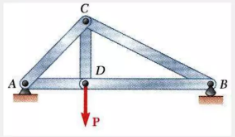
\includegraphics[height=2cm]{../images/truss}\hspace{0.5em}
      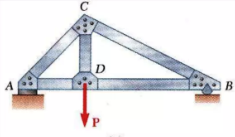
\includegraphics[height=2cm]{../images/truss1}
    \end{column}

    \begin{column}{0.42\textwidth}
      \centering
      \vspace{0.5cm}
      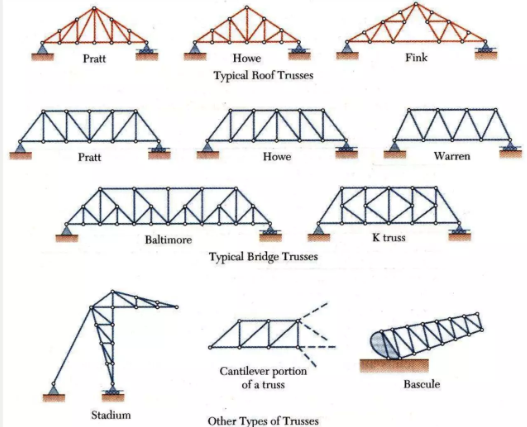
\includegraphics[width=\linewidth,height=0.78\textheight,keepaspectratio]{../images/truss3}
    \end{column}
  \end{columns}
\end{frame}

\begin{frame}{Kinematic assumptions}
  Trusses are assumed to exhibit the following characteristics:
  \begin{itemize}
    \item they experience either \textbf{compressive} or \textbf{tensile forces},
    \item their weight is considered negligible in comparison to the  loads they support,
    \item they have varying orientations with respect to a fixed global coordinate system, which serves as a stationary reference framework that remains unchanged regardless of the orientation of individual elements.
  \end{itemize}
  \begin{columns}
    \column{0.5\textwidth}
    \centering
    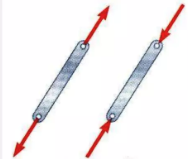
\includegraphics[height=2.3cm]{../images/truss2}

    \column{0.5\textwidth}
    \begin{tikzpicture}[scale=0.9]
      % Draw background grid
      %\draw[step=1cm,gray,very thin] (0,0) grid (12,6);
      % Define coordinates
      \coordinate (A) at (0,0);
      \coordinate (B) at (2.5,1);
      \coordinate (C) at (5,2);
      % Draw the truss members
      \draw[ultra thin] (A) -- (B);
      \draw[thick] (B) -- (C);
      % Global coordinate system
      \draw[-latex, ultra thin] (0,0) -- (0,3) node[left] {$y$};
      \draw[-latex, ultra thin] (0,0) -- (6,0) node[below] {$x$};
      % Nodes coord
      \draw[dashed,ultra thin] (B) -- (2.5,0) node[below] {$x_1$};
      \draw[dashed,ultra thin] (B) -- (0,1) node[left] {$y_1$};
      \draw[dashed,ultra thin] (C) -- (5,0) node[below] {$x_2$};
      \draw[dashed,ultra thin] (C) -- (0,2) node[left] {$y_2$};
      % Angles and labels
      \draw (1,0) arc (0:21.8:1);
      \node at (1.3,0.25) {$\theta$};
      % Local x' axis
      % Draw supports (circles at joints)
      \filldraw (B) circle (2pt);
      \filldraw (C) circle (2pt);
    \end{tikzpicture}
  \end{columns}
\end{frame}

\begin{frame}{Equation of motion for a single non-oriented bar element}
  \begin{columns}
    \column{0.7\textwidth}
    \begin{center}
      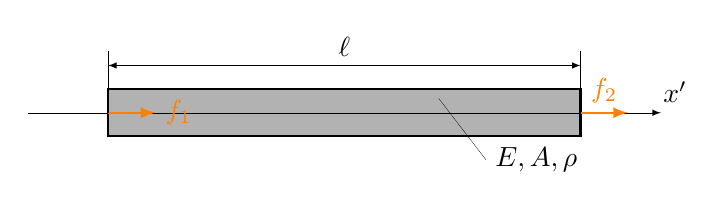
\begin{tikzpicture}[scale=0.6]
        % Draw the rectangle
        \filldraw[fill=gray!60, draw=black,thick] (0,-0.5) rectangle (10,0.5);
        %axis
        \draw[-latex, ultra thin] (-1.7,0) -- (11.7,0);
        \node[above] at (12,0) {\(x^\prime\)};
        \draw[thick,-latex,orange] (0,0) -- (1,0) node[right]{$f_{1}$};
        \draw[thick,-latex,orange] (10,0) -- (11,0) node[midway, above]{$f_{2}$};
        % length
        \draw[ultra thin] (10,0) -- (10, 1.3) ;
        \draw[ultra thin] (0,0) -- (0, 1.3) ;
        \draw[latex-latex, ultra thin]  (0,1)  to node[sloped,midway,above] {$\ell$}(10,1) ;
        \draw[ultra thin]  (7,0.3) -- (8,-1) node[right]{$E,A,\rho$};
      \end{tikzpicture}
    \end{center}

    \column{0.4\textwidth}
    {\tiny \begin{itemize}
        \item $A$ cross-sectional area
        \item $\ell$ length
        \item $E$ Young's modulus (isotropic bar)
        \item $\rho$ material density
        \item $u$ axial displacement
        \item $x^\prime$ (local) axial coordinate
      \end{itemize}}
  \end{columns}
  \vspace{0.3cm}

  \begin{itemize}
    \item Strong form:
          $$\begin{cases}
              \partial_{x^\prime}\left(EA \partial_{x^\prime}u(x^\prime, t)\right) = \rho A \ddot{u}(x^\prime, t) \\
              EA\partial_{x^\prime} u(0, t) = -f_{1}(t)                                                           \\
              EA\partial_{x^\prime} u(\ell, t) = f_{2}(t)                                                         \\
            \end{cases}\hspace{2cm}
            \begin{cases}
              u(x^\prime, 0) =  u_0(x^\prime)      \\
              \dot{u}(x^\prime, 0) = v_0(x^\prime) \\
            \end{cases}$$
    \item Semi-discrete weak form:
          \[\bolddelta\mathbf{q}_{loc}^T\big[\mathbf{M}_{loc} \ddot{\mathbf{q}}_{loc}(t) + \mathbf{K}_{loc} \mathbf{q}_{loc}(t) - \mathbf{f}_{loc}(t)\big]=0 \]
  \end{itemize}
\end{frame}

\begin{frame}{Approximated displacements in local coordinates}
  \begin{columns}
    \column{0.5\textwidth}
    \begin{center}
      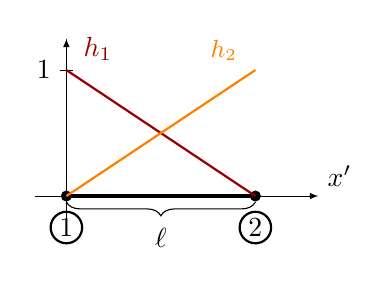
\begin{tikzpicture}[scale=0.8]
        % Define points
        \coordinate (A) at (0, 0);
        \coordinate (B) at (3, 0);
        % Mark points
        \fill (A) circle (2.5pt);
        \fill (B) circle (2.5pt);
        % Label the element
        \draw[ultra thick] (A) --(B);
        \draw[thick] (A) ++ (0,-0.5) circle(0.25cm) node {1};
        \draw[thick] (B) ++ (0,-0.5)  circle(0.25cm) node {2};
        %Axis 
        \draw[-latex,ultra thin] (-0.5,0) --(4,0) node[above right]{$x^\prime$};
        \draw[-latex, ultra thin] (0,-0.5) -- (0,2.5);
        \draw[ultra thin] (-.1,2) node[left] {$1$} -- (.1,2);
        %Draw functions 
        \draw[thick, darkred,domain=0:3, smooth, variable=\x]
        plot ({\x}, {(2-2*\x/3)});
        \draw[thick, orange,domain=0:3, smooth, variable=\x]
        plot ({\x}, {(2*\x/3)});
        \node[darkred, above] at (0.5, 2) {$h_1$};
        \node[orange, above] at (2.5, 2) {\small $h_2$};
        \draw [decorate,decoration={brace,amplitude=5pt,mirror,raise=0.5ex}]
        (A) -- (B) node[midway,yshift=-1.5em]{$\ell$};
      \end{tikzpicture}
    \end{center}

    \column{0.5\textwidth}
    \textbf{Linear local shape functions:}
    \begin{flalign*}
      h_1(x^\prime) & =1-\frac{x^\prime}{\ell} &  & \\
      h_2(x^\prime) & =\frac{x^\prime}{\ell}   &  &
    \end{flalign*}
  \end{columns}
  \vspace{0.2cm}
  \begin{itemize}
    \item Displacements approximation local coordinates:
          \[u^h(x^\prime,t)=  h_1(x^\prime) q_1(t)+h_2(x^\prime) q_2(t)=\begin{bmatrix}  h_1(x^\prime) & h_2(x^\prime)\end{bmatrix} \begin{bmatrix}  q_1(t) \\ q_2(t)\end{bmatrix}\]
    \item Virtual displacements approximation local coordinates:
          \[\delta u^h(x^\prime)=  h_1(x^\prime)\delta q_1+h_2(x^\prime)\delta q_2=\begin{bmatrix}  h_1(x^\prime) & h_2(x^\prime)\end{bmatrix} \begin{bmatrix} \delta q_1 \\ \delta q_2\end{bmatrix}\]
  \end{itemize}
\end{frame}


\begin{frame}{Elementary quantities in local coordinates}
  \begin{itemize}
    \item Element stiffness matrix in local coordinates:
          \[ \mathbf{K}_{loc} =\int_0^{\ell}  EA \begin{bmatrix} (h_1^\prime)^2 & h_1^\prime h_2^\prime \\  h_2^\prime h_1^\prime &  (h_2^\prime)^2 \end{bmatrix} dx^\prime =\frac{EA}{\ell} \begin{bmatrix} 1 & -1 \\ -1 & 1 \end{bmatrix} \]
    \item Element consistent mass matrix in local coordinates:
          \[ \mathbf{M}_{loc} =\int_0^{\ell}\rho A \begin{bmatrix} (h_1)^2 &h_1 h_2 \\  h_2 h_1 &  (h_2)^2 \end{bmatrix} dx^\prime =\frac{\rho A\ell }{6} \begin{bmatrix} 2 & 1 \\ 1 & 2 \end{bmatrix} \]
    \item Element applied loads vector in local coordinates:
          \[ \mathbf{f}_{loc}(t) =\begin{bmatrix} h_1(0) \\ h_2(0)\end{bmatrix}f_{1}(t) + \begin{bmatrix} h_1(\ell) \\ h_2(\ell)\end{bmatrix}f_{2}(t) = \begin{bmatrix} f_{1}(t) \\ f_{2}(t) \end{bmatrix} \]
  \end{itemize}
\end{frame}

\begin{frame}{Displacements for a single oriented bar}
  \begin{columns}
    \column{0.5\textwidth}
    \begin{itemize}
      \item Displacement vector in local coordinates:\vspace{-0.3cm}  $${\color{orange}\mathbf{q}_{loc}}= [q_1, q_2]^T.$$
      \item Displacement vector in global coordinates:\vspace{-0.3cm} $${\color{darkred}\mathbf q}= [q_{1x},q_{1y},q_{2x},q_{2y}]^T.$$
    \end{itemize}
    \column{0.5\textwidth}
    \begin{center}
      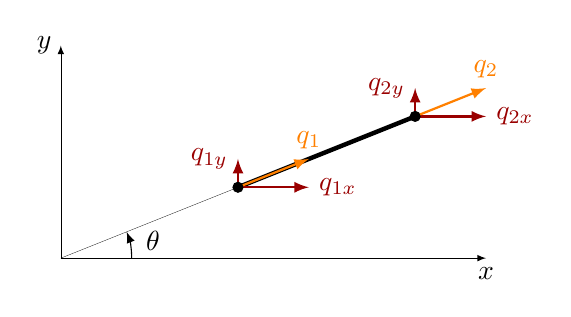
\begin{tikzpicture}[scale=0.9]
        % Draw background grid
        %\draw[step=1cm,gray,very thin] (0,0) grid (12,6);
        % Define coordinates
        \coordinate (A) at (0,0);
        \coordinate (B) at (2.5,1);
        \coordinate (C) at (5,2);
        % Draw the truss members
        \draw[ultra thin] (A) -- (B);
        \draw[ultra thick] (B) -- (C);
        % Global coordinate system
        \draw[-latex, ultra thin] (0,0) -- (0,3) node[left] {$y$};
        \draw[-latex, ultra thin] (0,0) -- (6,0) node[below] {$x$};
        % Local coordinate systems
        \draw[-latex, darkred,thick] (B) -- ++(0,0.4) node[left] {$q_{1y}$};
        \draw[-latex, darkred,thick] (B) -- ++(1,0) node[right] {$q_{1x}$};
        \draw[-latex, darkred,thick] (C) -- ++(0,0.4) node[left] {$q_{2y}$};
        \draw[-latex, darkred,thick] (C) -- ++(1,0) node[right] {$q_{2x}$};
        % Angles and labels
        \draw[-latex] (1,0) arc (0:21.8:1);
        \node at (1.3,0.25) {$\theta$};
        % Local x' axis
        \draw[-latex, orange, thick] (B) -- ++(1,0.4) node[above] {$q_1$};
        \draw[-latex, orange, thick] (C) -- ++(1,0.4) node[above] {$q_2$};
        % Draw supports (circles at joints)
        \filldraw (B) circle (2pt);
        \filldraw (C) circle (2pt);
      \end{tikzpicture}
    \end{center}
  \end{columns}
  \vspace{0.3cm}
  Relation between local and global displacements:
  $$\underbrace{\begin{bmatrix}
        q_1 \\ q_2
      \end{bmatrix}}_\text{$\mathbf q_{loc}$}=\underbrace{\begin{bmatrix}
        \cos(\theta) & \sin(\theta) & 0            & 0            \\
        0            & 0            & \cos(\theta) & \sin(\theta)
      \end{bmatrix}}_\text{$\mathbf T$}\underbrace{\begin{bmatrix}
        q_{1x} \\ q_{1y} \\ q_{2x} \\ q_{2y}
      \end{bmatrix}}_\text{$\mathbf q$}
  $$
\end{frame}


\begin{frame}{Calculation of direction sines and cosines}
  \begin{center}
    \begin{tikzpicture}[scale=0.9]
      % Draw background grid
      %\draw[step=1cm,gray,very thin] (0,0) grid (12,6);
      % Define coordinates
      \coordinate (A) at (0,0);
      \coordinate (B) at (2.5,1);
      \coordinate (C) at (5,2);
      % Draw the truss members
      \draw[ultra thin] (A) -- (B);
      \draw[thick] (B) -- (C);
      % Global coordinate system
      \draw[-latex, ultra thin] (0,0) -- (0,3) node[left] {$y$};
      \draw[-latex, ultra thin] (0,0) -- (6,0) node[below] {$x$};
      % Nodes coord
      \draw[dashed,ultra thin] (B) -- (2.5,0) node[below] {$x_1$};
      \draw[dashed,ultra thin] (B) -- (0,1) node[left] {$y_1$};
      \draw[dashed,ultra thin] (C) -- (5,0) node[below] {$x_2$};
      \draw[dashed,ultra thin] (C) -- (0,2) node[left] {$y_2$};
      % Angles and labels
      \draw[-latex] (1,0) arc (0:21.8:1);
      \node at (1.3,0.25) {$\theta$};
      % Local x' axis
      % Draw supports (circles at joints)
      \filldraw (B) circle (2pt);
      \filldraw (C) circle (2pt);
    \end{tikzpicture}
  \end{center}
  The direction sines and cosines can be calculated from the element
  geometry:
  \begin{align*}
    \sin(\theta) & = \frac{y_2-y_1}{\ell}          \\
    \cos(\theta) & = \frac{x_2-x_1}{\ell}          \\
    \ell         & =\sqrt{(x_2-x_1)^2+(y_2-y_1)^2}
  \end{align*}
\end{frame}


{\setbeamercolor{background canvas}{bg=darkred}
\setbeamercolor{block body}{bg=darkred,fg=white}
\setbeamercolor{itemize item}{fg=white}
\setbeamercolor{itemize/enumerate body}{fg=white}
\color{white}
\begin{frame}{Element stiffness and consistent mass matrices in global coordinates}
  \begin{itemize}
    \item Element stiffness matrix in global coordinates:
          \begin{align*}
            \mathbf{K} & = \mathbf T^T \mathbf{K}_{loc} \mathbf T                                                                          \\
                       & =\frac{EA}{\ell}\begin{bmatrix}
                                           \cos^2(\theta) & \sin(\theta)\cos(\theta) & -\cos^2(\theta)           & -\sin(\theta)\cos(\theta) \\
                                                          & \sin^2(\theta)           & -\sin(\theta)\cos(\theta) & -\sin^2(\theta)           \\
                                                          &                          & \cos^2(\theta)            & \sin(\theta)\cos(\theta)  \\
                                           \text{Symm.}   &                          &                           & \sin^2(\theta)            \\
                                         \end{bmatrix}
          \end{align*}
    \item Element consistent mass matrix in global coordinates:
          \begin{align*}
            \mathbf{M} & = \mathbf T^T \mathbf{M}_{loc} \mathbf T                                                                                \\
                       & =\frac{\rho A\ell}{6}\begin{bmatrix}
                                                2\cos^2(\theta) & 2\sin(\theta)\cos(\theta) & \cos^2(\theta)           & \sin(\theta)\cos(\theta)  \\
                                                                & 2\sin^2(\theta)           & \sin(\theta)\cos(\theta) & \sin^2(\theta)            \\
                                                                &                           & 2\cos^2(\theta)          & 2\sin(\theta)\cos(\theta) \\
                                                \text{Symm.}    &                           &                          & 2\sin^2(\theta)           \\
                                              \end{bmatrix}
          \end{align*}
  \end{itemize}
\end{frame}

\begin{frame}{Lumped mass matrix}
  \begin{itemize}
    \item Element consistent mass matrix in local coordinates:
          \[ \mathbf{M}_{loc} =\frac{\rho A\ell }{6} \begin{bmatrix} 2 & 1 \\ 1 & 2 \end{bmatrix} \]
    \item Element lumped mass matrix in local coordinates:
          \[ \mathbf{M}_{loc} =\frac{\rho A\ell }{2} \begin{bmatrix} 1 & 0 \\ 0 & 1 \end{bmatrix} \]
    \item Element lumped mass matrix in global coordinates:
          \begin{align*}
            \mathbf{M} & = \mathbf T^T \mathbf{M}_{loc} \mathbf T                                                                                       \\
                       & =\frac{\rho A\ell}{2}\begin{bmatrix}
                                                \cos^2(\theta)           & \sin(\theta)\cos(\theta) & 0                        & 0                        \\
                                                \sin(\theta)\cos(\theta) & \sin^2(\theta)           & 0                        & 0                        \\
                                                0                        & 0                        & \cos^2(\theta)           & \sin(\theta)\cos(\theta) \\
                                                0                        & 0                        & \sin(\theta)\cos(\theta) & \sin^2(\theta)           \\
                                              \end{bmatrix}
          \end{align*}
  \end{itemize}
\end{frame}
}

\begin{frame}{Benefits of using lumped mass matrix}

  \begin{itemize}
    \item[\Checkmark] \textbf{Computational efficiency}
          \begin{itemize}
            \item[] Band matrix for faster computations and lower memory usage.
          \end{itemize}

    \item[\Checkmark] \textbf{Improved numerical stability}
          \begin{itemize}
            \item[] Help avoid non-physical coupling between DOFs, which can cause instabilities, in explicit time integration (Newmark or central difference methods).
          \end{itemize}

    \item[\Checkmark] \textbf{Physical realism for trusses}
          \begin{itemize}
            \item[] Truss mass is mostly at joints so lumped mass better reflects reality.
          \end{itemize}

    \item[\Checkmark] \textbf{Good approximation in practice}
          \begin{itemize}
            \item[] Accurate enough for natural frequency and mode shape estimation.
          \end{itemize}
  \end{itemize}
  \vspace{0.3cm}

  \begin{tcolorbox}[colback=darkred!10,colframe=darkred!40!black]
    \begin{center}
      \textit{Band mass matrix = faster, simpler, and often accurate enough!}
    \end{center}
  \end{tcolorbox}
\end{frame}

\begin{frame}{Applied loads for a single oriented bar}
  \begin{columns}
    \column{0.5\textwidth}
    \begin{itemize}
      \item Nodal force vector in local coordinates:\vspace{-0.3cm}$${\color{orange}\mathbf{f}_{loc}} = [f_{1}, f_{2}]^T.$$
      \item Nodal force vector in global coordinates:\vspace{-0.3cm} $${\color{darkred}\mathbf{f}} = [f_{1x}, f_{1y}, f_{2x}, f_{2y}]^T.$$
    \end{itemize}
    \column{0.5\textwidth}
    \begin{center}
      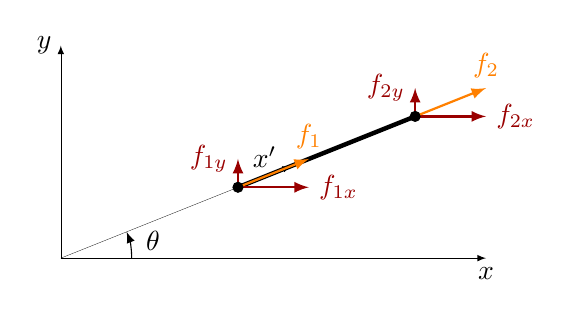
\begin{tikzpicture}[scale=0.9]
        % Draw background grid
        %\draw[step=1cm,gray,very thin] (0,0) grid (12,6);
        % Define coordinates
        \coordinate (A) at (0,0);
        \coordinate (B) at (2.5,1);
        \coordinate (C) at (5,2);
        % Draw the truss members
        \draw[ultra thin] (A) -- (B);
        \draw[ultra thick] (B) -- (C);
        % Global coordinate system
        \draw[-latex, ultra thin] (0,0) -- (0,3) node[left] {$y$};
        \draw[-latex, ultra thin] (0,0) -- (6,0) node[below] {$x$};
        % Local coordinate systems
        \draw[-latex, darkred,thick] (B) -- ++(0,0.4) node[left] {$f_{1y}$};
        \draw[-latex, darkred,thick] (B) -- ++(1,0) node[right] {$f_{1x}$};
        \draw[-latex, darkred,thick] (C) -- ++(0,0.4) node[left] {$f_{2y}$};
        \draw[-latex, darkred,thick] (C) -- ++(1,0) node[right] {$f_{2x}$};
        % Local primed coordinate system
        \draw[-latex,ultra thin] (B) -- (21.8:3.5) node[midway,above] {$x^\prime$};
        % Angles and labels
        \draw[-latex] (1,0) arc (0:21.8:1);
        \node at (1.3,0.25) {$\theta$};
        % Local x' axis
        \draw[-latex, orange, thick] (B) -- ++(1,0.4) node[above] {$f_{1}$};
        \draw[-latex, orange, thick] (C) -- ++(1,0.4) node[above] {$f_{2}$};
        % Draw supports (circles at joints)
        \filldraw (B) circle (2pt);
        \filldraw (C) circle (2pt);
      \end{tikzpicture}
    \end{center}
  \end{columns}
  \vspace{0.3cm}
  Forces undergo transformation in the same manner as displacements:
  $$\underbrace{\begin{bmatrix}
        f_{1} \\ f_{2}
      \end{bmatrix}}_\text{$\mathbf f_{loc}$}=\underbrace{\begin{bmatrix}
        \cos(\theta) & \sin(\theta) & 0            & 0            \\
        0            & 0            & \cos(\theta) & \sin(\theta)
      \end{bmatrix}}_\text{$\mathbf T$}\underbrace{\begin{bmatrix}
        f_{1x} \\ f_{1y} \\  f_{2x} \\  f_{2y}
      \end{bmatrix}}_\text{$\mathbf f$}
  $$
\end{frame}


\begin{frame}{Elementary loads vector in global coordinates}
  \begin{itemize}
    \item Element applied loads vector in global coordinates:
          \[
            \mathbf{f} = \mathbf T^T \mathbf{f}_{loc} =\begin{bmatrix}
              \cos(\theta)f_1 \\
              \sin(\theta)f_1 \\
              \cos(\theta)f_2 \\
              \sin(\theta)f_2 \\
            \end{bmatrix}
          \]
  \end{itemize}

  \vspace{0.5em}
  \begin{itemize}
    \item Loads are only applied at pins and are given in the global coordinates system, the assembled loads vector can be computed directly.
    \item Distributed/self-weight loads are transformed to equivalent nodal loads.
  \end{itemize}
\end{frame}


{\setbeamercolor{background canvas}{bg=darkred}
\setbeamercolor{block body}{bg=darkred,fg=white}
\setbeamercolor{itemize item}{fg=white}
\setbeamercolor{itemize/enumerate body}{fg=white}
\color{white}
\begin{frame}{Assembly of stiffness and mass matrices and loads vector}
  Given a 2d truss structure made of $m$ oriented bars, $n$ nodes.

  \vspace{0.5em}
  \textbf{1. Element quantities:}
  \begin{itemize}
    \item For each bar element $e$, compute the element quantities global coordinates:
          \begin{align*}
            {}^e\mathbf{K} & ={}^e\mathbf{T}^{T} {}^e\mathbf{K}_{loc}{}^e\mathbf{T} \\
            {}^e\mathbf{M} & ={}^e\mathbf{T}^{T} {}^e\mathbf{M}_{loc}{}^e\mathbf{T} \\
            {}^e\mathbf{f} & ={}^e\mathbf{T}^{T} {}^e\mathbf{f}_{loc}
          \end{align*}
  \end{itemize}

  \vspace{0.5em}
  \textbf{2. Global assembly:}
  \begin{itemize}
    \item Initialize global stiffness matrix $\mathbf{K}$ and global mass matrix $\mathbf{M}$ of size $2n \times 2n$.
    \item  Initialize global loads vector $\mathbf{f}$ of size $2n \times 1$.
    \item Assemble each ${}^e\mathbf{K}$, ${}^e\mathbf{M}$ and ${}^e\mathbf{f}$ for $e=1,\dots,m$, into $\mathbf{K}$, $\mathbf{M}$ and $\mathbf{f}$ respectively using element connectivity.
  \end{itemize}
\end{frame}
}

\begin{frame}{Reduced stiffness and mass matrices and loads vector}
  \textbf{3. Boundary conditions:}
  \begin{itemize}
    \item Identify constrained (\emph{fixed or supported}) degrees of freedom,
    \item Partition global matrices and vectors to separate free and constrained DOFs:
          \[
            \mathbf{K} = \begin{bmatrix}
              \mathbf{K}_{ff} & \mathbf{K}_{fc} \\
              \mathbf{K}_{cf} & \mathbf{K}_{cc}
            \end{bmatrix}, \quad
            \mathbf{M} = \begin{bmatrix}
              \mathbf{M}_{ff} & \mathbf{M}_{fc} \\
              \mathbf{M}_{cf} & \mathbf{M}_{cc}
            \end{bmatrix}, \quad
            \mathbf{f} = \begin{bmatrix}
              \mathbf{f}_{f} \\
              \mathbf{f}_{c}
            \end{bmatrix}.
          \]
    \item Apply constraints by removing or modifying rows and columns corresponding to constrained DOFs.
  \end{itemize}
  \begin{columns}[T,onlytextwidth]
    % Pin and roller
    \begin{column}{0.33\textwidth}
      \centering
      \textbf{Pin--roller}

      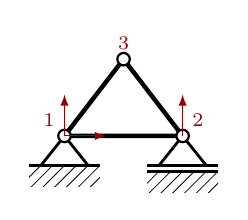
\begin{tikzpicture}[scale=0.75, every node/.style={font=\scriptsize}]
        \coordinate (1) at (0,0);
        \coordinate (2) at (2,0);
        \coordinate (3) at (1,1.3);

        \point{a}{0}{0};
        \point{b}{1.5}{0};
        \support{1}{a}[0];
        \support{2}{b}[0];

        \draw[ultra thick] (1)--(2)--(3)--cycle;
        \foreach \p in {1,2,3}
        \draw[thick,fill=white] (\p) circle (3pt);

        \node[above left,darkred] at (1) {1};
        \node[above right,darkred] at (2) {2};
        \node[above,darkred] at (3) {3};

        \draw[-latex,thin,darkred] (1) -- ++(0.7,0);
        \draw[-latex,thin,darkred] (1) -- ++(0,0.7);
        \draw[-latex,thin,darkred] (2) -- ++(0,0.7);
      \end{tikzpicture}

      \scriptsize Pin: $q_{1x}=q_{1y}=0$; \\ roller: $q_{2y}=0$.
    \end{column}

    % Two pinned supports
    \begin{column}{0.33\textwidth}
      \centering
      \textbf{Pin-pin}

      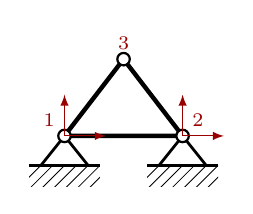
\begin{tikzpicture}[scale=0.75, every node/.style={font=\scriptsize}]
        \coordinate (1) at (0,0);
        \coordinate (2) at (2,0);
        \coordinate (3) at (1,1.3);

        \point{a}{0}{0};
        \point{b}{1.5}{0};
        \support{1}{a}[0];
        \support{1}{b}[0];

        \draw[ultra thick] (1)--(2)--(3)--cycle;
        \foreach \p in {1,2,3}
        \draw[thick,fill=white] (\p) circle (3pt);

        \node[above left,darkred] at (1) {1};
        \node[above right,darkred] at (2) {2};
        \node[above,darkred] at (3) {3};

        \draw[-latex,thin,darkred] (1) -- ++(0.7,0);
        \draw[-latex,thin,darkred] (1) -- ++(0,0.7);
        \draw[-latex,thin,darkred] (2) -- ++(0,0.7);
        \draw[-latex,thin,darkred] (2) -- ++(0.7,0);
      \end{tikzpicture}

      \scriptsize Pin: $q_{1x}=q_{1y}=0$; \\ Pin: $q_{2x}=q_{2y}=0$.
    \end{column}

    % Cantilever
    \begin{column}{0.33\textwidth}
      \centering
      \textbf{Pin-free}

      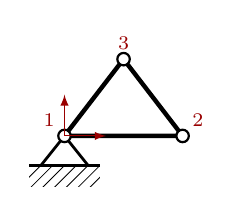
\begin{tikzpicture}[scale=0.75, every node/.style={font=\scriptsize}]
        \coordinate (1) at (0,0);
        \coordinate (2) at (2,0);
        \coordinate (3) at (1,1.3);

        \point{a}{0}{0};
        \support{1}{a}[0];

        \draw[ultra thick] (1)--(2)--(3)--cycle;
        \foreach \p in {1,2,3}
        \draw[thick,fill=white] (\p) circle (3pt);

        \node[above left,darkred] at (1) {1};
        \node[above right,darkred] at (2) {2};
        \node[above,darkred] at (3) {3};

        \draw[-latex,thin,darkred] (1) -- ++(0.7,0);
        \draw[-latex,thin,darkred] (1) -- ++(0,0.7);
      \end{tikzpicture}

      \scriptsize Pin: $q_{1x}=q_{1y}=0$.
    \end{column}
  \end{columns}
\end{frame}

\begin{frame}{Modal analysis}
  \begin{itemize}
    \item Solve the free vibrations (homogeneous) problem without external loads:
          \[
            \mathbf{M}_{ff} \ddot{\mathbf{q}}_f(t) + \mathbf{K}_{ff} \mathbf{q}_f(t) = \mathbf{0}.
          \]
    \item Assume harmonic motion $\mathbf{q}_f(t) = \boldsymbol{\phi} \, e^{i \omega t}$ and derive the eigenvalue problem:
          \[
            \left( \mathbf{K}_{ff} - \omega^2 \mathbf{M}_{ff} \right) \boldsymbol{\phi} = \mathbf{0}.
          \]
    \item Solve for eigenvalues $\lambda=\omega^2$ (squared natural frequencies):
          \[
            \det\left( \mathbf{K}_{ff} - \lambda \mathbf{M}_{ff} \right) = 0.
          \]
    \item Solve for corresponding eigenvectors $\boldsymbol{\phi}$ (mode shapes). Normalize eigenvectors with respect to $\mathbf{M}_{ff}$ or $\mathbf{K}_{ff}$.
  \end{itemize}
\end{frame}

\begin{frame}{Transient analysis}
  \begin{itemize}
    \item The dynamic equilibrium equation for the free DOFs becomes:
          \[
            \mathbf{M}_{ff} \ddot{\mathbf{q}}_{f}(t) + \mathbf{K}_{ff} \mathbf{q}_{f}(t) = \mathbf{f}_{f}(t).
          \]
    \item This coupled system of equations can be uncoupled by transforming to modal coordinates using the normal mode matrix $\boldsymbol{\Phi}$, where $\mathbf{q}_f(t) = \boldsymbol{\Phi} \mathbf{z}(t)$.
    \item Substituting into the equation and pre-multiplying by $\boldsymbol{\Phi}^T$, we obtain a decoupled system:
          \[
            \ddot{\mathbf{z}}(t) + \boldsymbol{\Lambda} \mathbf{z}(t) = \boldsymbol{\Phi}^T \mathbf{f}_f(t),
          \]
          where $\boldsymbol{\Lambda}$ is a diagonal matrix of squared natural frequencies.
    \item The decoupled equations in modal space can be solved independently using time integration methods, greatly simplifying the dynamic analysis.
  \end{itemize}
\end{frame}

\begin{frame}{Post-processing: stress computation}
  \begin{itemize}
    \item In the local coordinate system, the approximated axial stress in element $e$ is
          $${}^e\sigma^h_{loc}=E{}^e\varepsilon_{loc}^h$$
    \item Stain-displacement relationship:
          $${}^e\varepsilon_{loc}^h=\frac{d}{dx^\prime}u^h= \begin{bmatrix}  \dfrac{d h_1}{dx^\prime}  & \dfrac{d h_2}{dx^\prime} \end{bmatrix} \begin{bmatrix}  q_1 \\ q_2\end{bmatrix}=\frac{1}{{}^e\ell}\begin{bmatrix} -1  & 1 \end{bmatrix} \begin{bmatrix}  q_1 \\ q_2\end{bmatrix}$$
    \item Using the coordinate transformation ${}^e\mathbf q_{loc}={}^e\mathbf T\mathbf q$ it leads to the approximated stress computed in global coordinates:\vspace{-0.3cm}
          \begin{align*}
            {}^e\sigma^h & =\frac{{}^eE}{{}^e\ell}\begin{bmatrix} -\cos({}^e\theta)  & -\sin({}^e\theta) & \cos({}^e\theta) & \sin({}^e\theta) \end{bmatrix} \begin{bmatrix}
                                                                                                                                                               q_{ix} \\ q_{iy} \\ q_{jx} \\ q_{jy}
                                                                                                                                                             \end{bmatrix} \\
                         & =
            \frac{{}^eE}{{}^e\ell} \left[
              \cos({}^e\theta)(q_{jx} - q_{ix}) + \sin({}^e\theta)(q_{jy} - q_{iy})
              \right]
          \end{align*}
          Note that element $e$ is connected to nodes numbered as $i$ and $j$.
  \end{itemize}
\end{frame}

\section{Illustrative example of a 2d truss structure}

\begin{frame}{Problem description}
  \begin{columns}
    \begin{column}{.45\textwidth}
      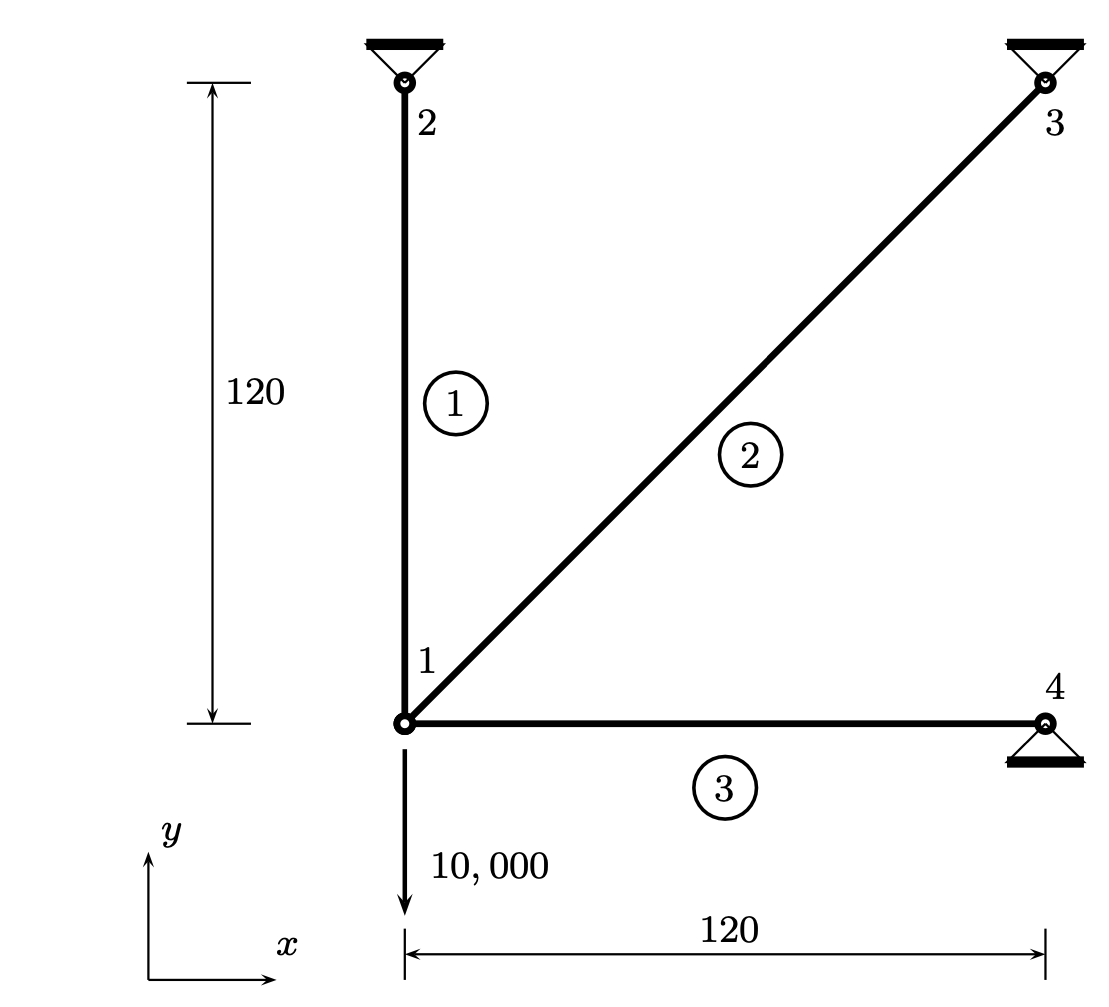
\includegraphics[width=6.5cm]{../images/trussExample.png}
    \end{column}

    \begin{column}{.53\textwidth}
      Magnesium alloy material properties:
      \begin{itemize}
        \item cross-sectional area $A=78.5$ mm${}^2$
        \item Young's modulus $E=40\cdot 10^{3}$ MPa
        \item Density $\rho=1.810$ ton/m${}^3$
      \end{itemize}
      Parameters:
      \vspace{0.2cm}

      \begin{tabular}{c|c|c|c}
        Elements & Nodes & ${}^e\theta$  & ${}^e\ell$       \\
        \hline
        1        & 1,\ 2 & $90^{\circ}$  & $120$ mm         \\
        2        & 1,\ 3 & $45^{\circ} $ & $120\sqrt{2}$ mm \\
        3        & 1,\ 4 & $0^{\circ} $  & $120$ mm         \\
      \end{tabular}
    \end{column}
  \end{columns}
  \begin{block}{}
    \textbf{Objective:} Compute the equation of motion in semi-discrete weak form.
  \end{block}
  \noindent{\tiny\emph{Credit: Ferreira and Fantuzzi, MATLAB Codes for Finite Element Analysis}}
\end{frame}

\begin{frame}{Element matrices in global coordinates}
  \vspace{-0.7cm}
  \begin{itemize}
    \item     \small\textbf{Element stiffness matrices}
  \end{itemize}
  \vspace{0.1cm}
  {\centering
  \resizebox{\textwidth}{!}{$\displaystyle
    {}^1\mathbf{K}
    = {}^1\mathbf{T}^{T}\mathbf{K}_{\mathrm{loc}}{}^1\mathbf{T}
    = \frac{EA}{{}^1\ell}
    \begin{bmatrix}
      \cos(90^\circ) & 0              \\
      \sin(90^\circ) & 0              \\
      0              & \cos(90^\circ) \\
      0              & \sin(90^\circ)
    \end{bmatrix}
    \begin{bmatrix}
      1  & -1 \\
      -1 & 1
    \end{bmatrix}
    \begin{bmatrix}
      \cos(90^\circ) & \sin(90^\circ) & 0              & 0              \\
      0              & 0              & \cos(90^\circ) & \sin(90^\circ)
    \end{bmatrix}
    = \frac{78500}{3}
    \begin{bmatrix}
      0 & 0  & 0 & 0  \\
      0 & 1  & 0 & -1 \\
      0 & 0  & 0 & 0  \\
      0 & -1 & 0 & 1
    \end{bmatrix}
  $}
  }
  By analogy:
  $${}^2\mathbf{K} =
    \frac{78500}{6\sqrt{2}}
    \begin{bmatrix}
      1  & 1  & -1 & -1 \\
      1  & 1  & -1 & -1 \\
      -1 & -1 & 1  & 1  \\
      -1 & -1 & 1  & 1
    \end{bmatrix}\qquad {}^3\mathbf{K} =
    \frac{78500}{3}
    \begin{bmatrix}
      1  & 0 & -1 & 0 \\
      0  & 0 & 0  & 0 \\
      -1 & 0 & 1  & 0 \\
      0  & 0 & 0  & 0
    \end{bmatrix}
  $$
  \vspace{-0.3cm}
  \begin{itemize}
    \item     \small\textbf{Element consistent mass matrices}
  \end{itemize}
  \vspace{0.1cm}
  {\centering
    \resizebox{\textwidth}{!}{${}^1\mathbf{M} = \frac{28417}{10}
        \begin{bmatrix}
          0 & 0 & 0 & 0 \\
          0 & 2 & 0 & 1 \\
          0 & 0 & 0 & 0 \\
          0 & 1 & 0 & 2
        \end{bmatrix}
        \qquad
        {}^2\mathbf{M} =
        \frac{28417}{20}\sqrt{2}
        \begin{bmatrix}
          2 & 2 & 1 & 1 \\
          2 & 2 & 1 & 1 \\
          1 & 1 & 2 & 2 \\
          1 & 1 & 2 & 2
        \end{bmatrix}
        \qquad
        {}^3\mathbf{M} =
        \frac{28417}{10}
        \begin{bmatrix}
          2 & 0 & 1 & 0 \\
          0 & 0 & 0 & 0 \\
          1 & 0 & 2 & 0 \\
          0 & 0 & 0 & 0
        \end{bmatrix}
      $}}
\end{frame}

\begin{frame}{Assembly of the global stiffness and consistent mass matrices}
  \centering
  \scriptsize

  \begin{tabular}{c|c|c|c}
    Local index & {\color{darkred}bar 1} & {\color{orange}bar 2} & {\color{brown}bar 3} \\
    \hline
    1           & {\color{darkred}1}     & {\color{orange}1}     & {\color{brown}1}     \\
    2           & {\color{darkred}2}     & {\color{orange}3}     & {\color{brown}4}
  \end{tabular}

  \vspace{0.5cm}
  \textbf{Global stiffness matrix : }
  \resizebox{8cm}{!}{$\displaystyle
      \mathbf K=\frac{78500}{6}\begin{bmatrix}
        {\color{brown}2}+{\color{orange}1/\sqrt 2} & {\color{orange}1/\sqrt 2}                    & 0 & 0                   & {\color{orange}-1/\sqrt 2} & {\color{orange}-1/\sqrt 2} & {\color{brown}-2} & 0 \\
        {\color{orange}1/\sqrt 2}                  & {\color{darkred}2}+{\color{orange}1/\sqrt 2} & 0 & {\color{darkred}-2} & {\color{orange}-1/\sqrt 2} & {\color{orange}-1/\sqrt 2} & 0                 & 0 \\
        0                                          & 0                                            & 0 & 0                   & 0                          & 0                          & 0                 & 0 \\
        0                                          & {\color{darkred}-2}                          & 0 & {\color{darkred}2}  & 0                          & 0                          & 0                 & 0 \\
        {\color{orange}-1/\sqrt 2}                 & {\color{orange}-1/\sqrt 2}                   & 0 & 0                   & {\color{orange}1/\sqrt 2}  & {\color{orange}1/\sqrt 2}  & 0                 & 0 \\
        {\color{orange}-1/\sqrt 2}                 & {\color{orange}-1/\sqrt 2}                   & 0 & 0                   & {\color{orange}1/\sqrt 2}  & {\color{orange}1/\sqrt 2}  & 0                 & 0 \\
        {\color{brown}-2}                          & 0                                            & 0 & 0                   & 0                          & 0                          & {\color{brown}2}  & 0 \\
        0                                          & 0                                            & 0 & 0                   & 0                          & 0                          & 0                 & 0
      \end{bmatrix}
    $}

  \vspace{0.5cm}
  \textbf{Global mass matrix : }
  \resizebox{8cm}{!}{$\displaystyle
      \mathbf M=\frac{28417}{20}\begin{bmatrix}
        {\color{brown}4}+{\color{orange}2\sqrt 2} & {\color{orange}2\sqrt 2}                    & 0 & 0                  & {\color{orange}\sqrt 2}  & {\color{orange}\sqrt 2}  & {\color{brown}2} & 0 \\
        {\color{orange}2\sqrt 2}                  & {\color{darkred}4}+{\color{orange}2\sqrt 2} & 0 & {\color{darkred}2} & {\color{orange}\sqrt 2}  & {\color{orange}\sqrt 2}  & 0                & 0 \\
        0                                         & 0                                           & 0 & 0                  & 0                        & 0                        & 0                & 0 \\
        0                                         & {\color{darkred}2}                          & 0 & {\color{darkred}4} & 0                        & 0                        & 0                & 0 \\
        {\color{orange}-\sqrt 2}                  & {\color{orange}-\sqrt 2}                    & 0 & 0                  & {\color{orange}2\sqrt 2} & {\color{orange}2\sqrt 2} & 0                & 0 \\
        {\color{orange}\sqrt 2}                   & {\color{orange}\sqrt 2}                     & 0 & 0                  & {\color{orange}2\sqrt 2} & {\color{orange}2\sqrt 2} & 0                & 0 \\
        {\color{brown}2}                          & 0                                           & 0 & 0                  & 0                        & 0                        & {\color{brown}4} & 0 \\
        0                                         & 0                                           & 0 & 0                  & 0                        & 0                        & 0                & 0
      \end{bmatrix}
    $}
\end{frame}

\begin{frame}{Applied loads and boundary conditions}
  \begin{columns}
    \begin{column}{.35\textwidth}
      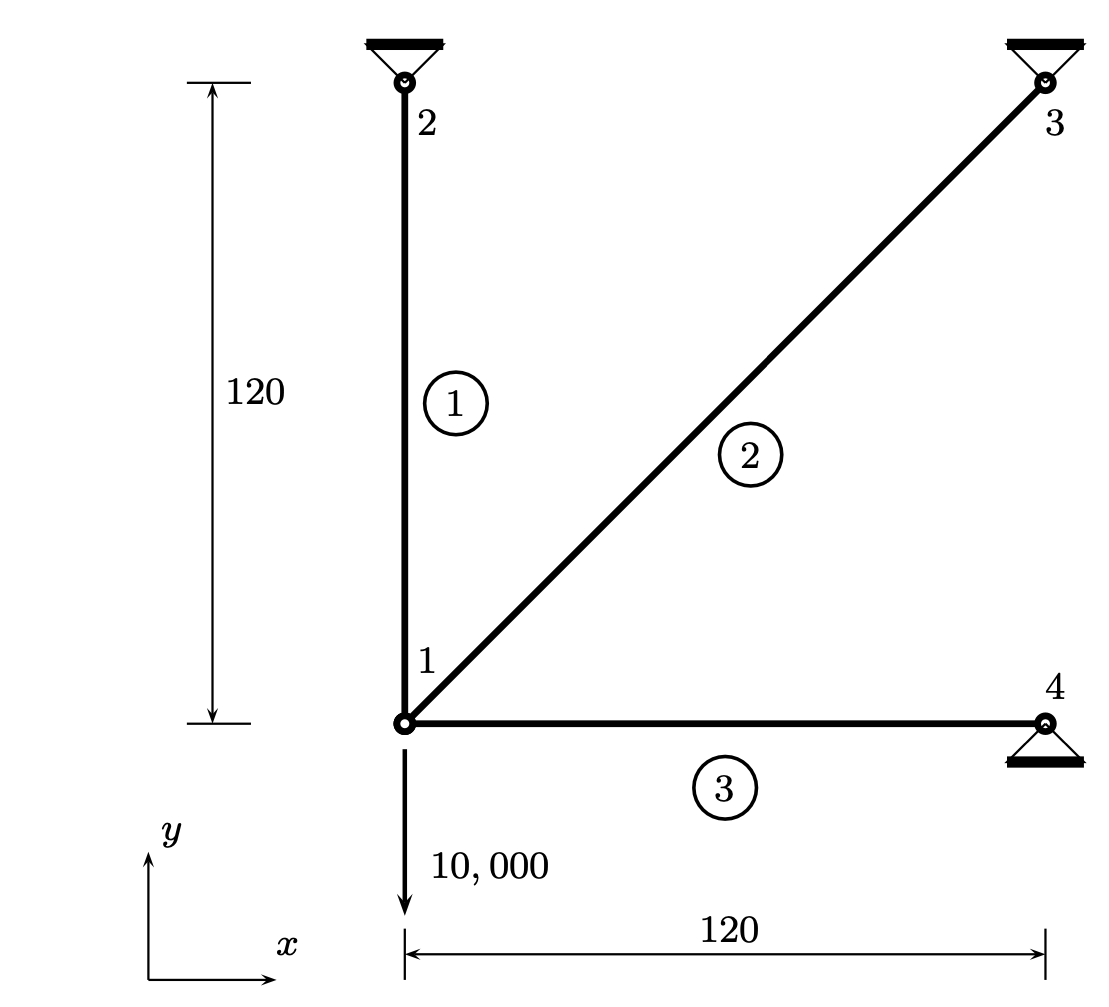
\includegraphics[width=4.5cm]{../images/trussExample.png}
    \end{column}

    \begin{column}{.3\textwidth}
      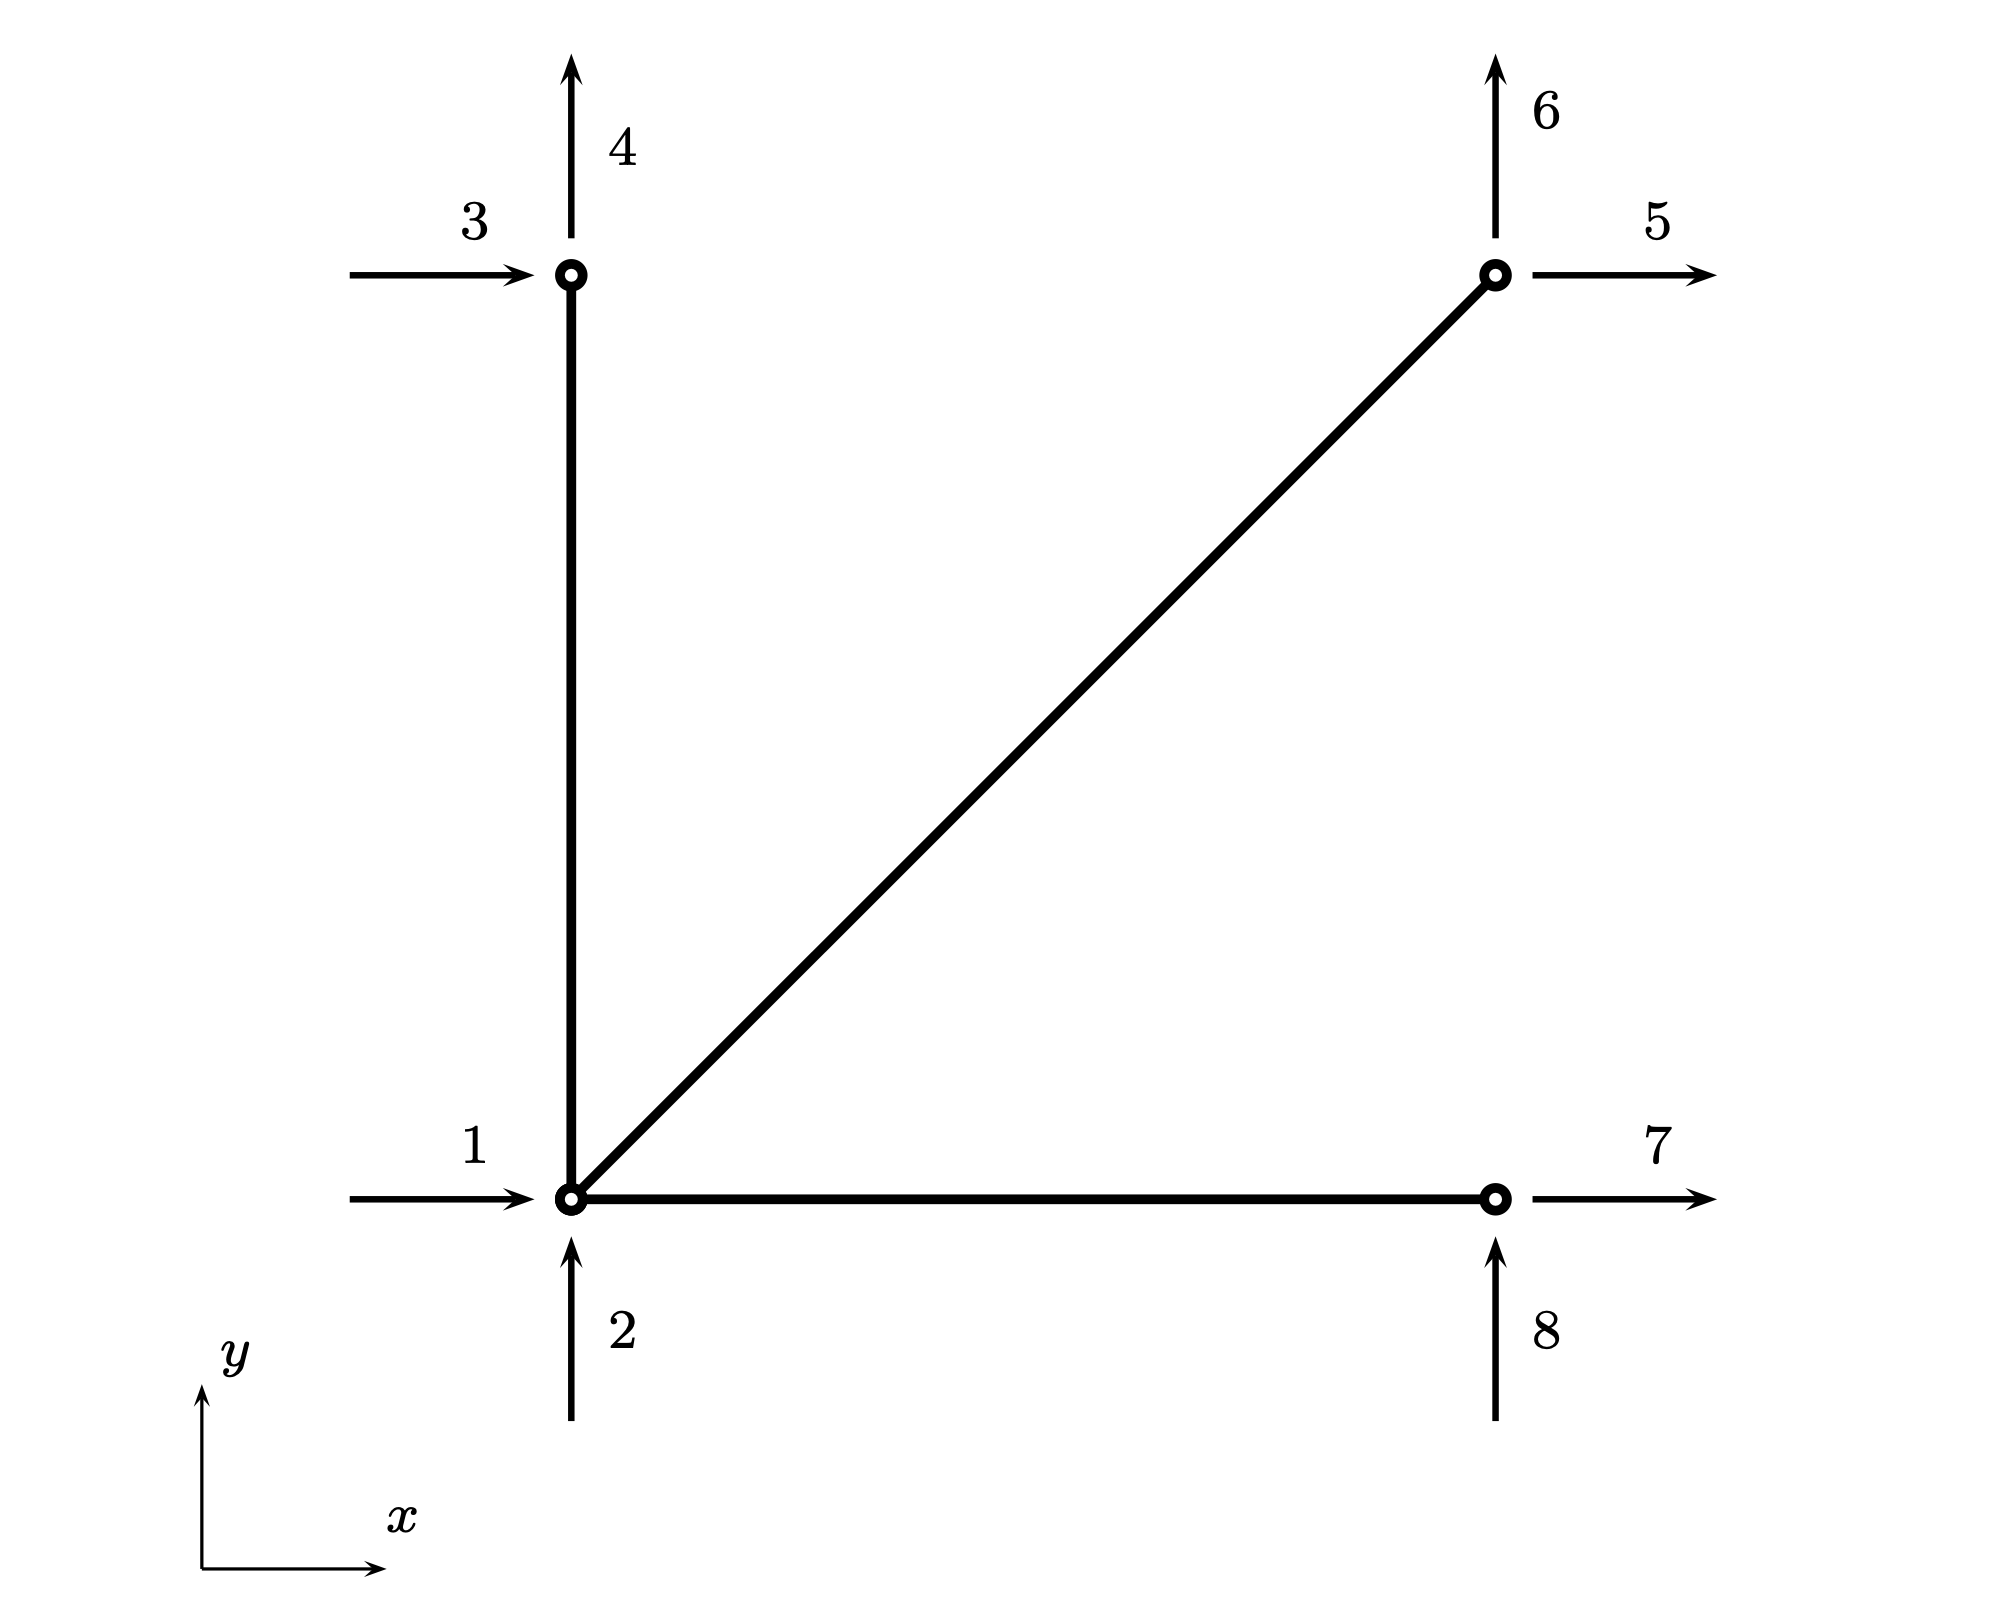
\includegraphics[width=4.5cm]{../images/trussExample1.png}
    \end{column}

    \begin{column}{.53\textwidth}
      $$\mathbf f=\begin{bmatrix}
          0 \\ -10000 \\ f_{2x} \\ f_{2y} \\ f_{3x} \\ f_{3y} \\ f_{4x} \\ f_{4y} \\
        \end{bmatrix} \qquad \mathbf q=\begin{bmatrix}
          q_{1x} \\ q_{1y} \\ 0 \\ 0 \\ 0 \\ 0 \\ 0 \\ 0
        \end{bmatrix}$$
    \end{column}
  \end{columns}
  \vspace{0.3cm}
  \begin{itemize}
    \item The free DOFs are $q_{1x}$ and $q_{1y}$.
  \end{itemize}
  The equations of motions for free nodes are given by :
  $${\frac{28417}{20}}\begin{bmatrix}
      4+2\sqrt{2} & 2\sqrt{2} \\
      2\sqrt{2} 4+2\sqrt{2}
    \end{bmatrix}\begin{bmatrix}
      \ddot{q}_{1x} \\ \ddot{q}_{1y}
    \end{bmatrix}+\frac{78500}{6}\begin{bmatrix}
      2+1/\sqrt{2} & 1/\sqrt{2}   \\
      1/\sqrt{2}   & 2+1/\sqrt{2}
    \end{bmatrix}\begin{bmatrix}
      q_{1x} \\ q_{1y}
    \end{bmatrix}=\begin{bmatrix}
      0 \\ -10000
    \end{bmatrix}$$

  \noindent{\tiny\emph{Credit: Ferreira and Fantuzzi, MATLAB Codes for Finite Element Analysis}}
\end{frame}

\begin{frame}{An example of a 2d truss in free vibration}
  \begin{center}
    \href{https://drive.mathworks.com/sharing/6a9792ef-d0a7-4aca-a1d0-8b1862b0ac3b}{\beamergotobutton{Go to Matlab Drive}}
  \end{center}
\end{frame}

\section{Trusses in 3d}
\begin{frame}{Displacements for oriented bar in 3d}
  \begin{columns}
    \column{0.5\textwidth}
    \begin{itemize}
      \item Displacements in local coord. does not change w.r.t the one in 2d:   $${\color{orange}\mathbf{q}_{loc}} = [q_1, q_2]^T.$$
      \item Displacements in global coordinates projected from nodes 1 and 2 have now 6 components: $${\color{darkred}\mathbf q} = [q_{1x},q_{1y},q_{1z},q_{2x},q_{2y},q_{2z}]^T.$$
    \end{itemize}
    \column{0.5\textwidth}
    \begin{center}
      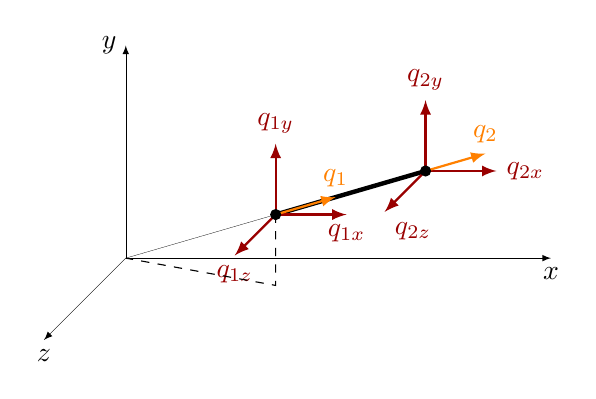
\begin{tikzpicture}[scale=0.9]
        % Draw background grid
        % Define coordinates
        \coordinate (A) at (0,0);
        \coordinate (B) at (2.5,1,1);
        \coordinate (C) at (5,2,2);
        % Draw the truss members
        \draw[ultra thin] (A) -- (B);
        \draw[ultra thick] (B) -- (C);
        % Global coordinate system
        \draw[-latex, ultra thin] (0,0) -- (0,3) node[left] {$y$};
        \draw[-latex, ultra thin] (0,0) -- (6,0) node[below] {$x$};
        \draw[-latex, ultra thin] (0,0) -- (0,0,3) node[below] {$z$};
        % Local coordinate systems
        \draw[-latex, darkred, thick] (B) -- ++(0,1) node[above] {$q_{1y}$};
        \draw[-latex, darkred, thick] (B) -- ++(1,0) node[below] {$q_{1x}$};
        \draw[-latex, darkred, thick] (B) -- ++(0,0,1.5) node[below] {$q_{1z}$};
        \draw[-latex, darkred, thick] (C) -- ++(0,1) node[above] {$q_{2y}$};
        \draw[-latex, darkred, thick] (C) -- ++(1,0) node[right] {$q_{2x}$};
        \draw[-latex, darkred, thick] (C) -- ++(0,0,1.5) node[below right] {$q_{2z}$};
        % Local x' axis
        \draw[-latex, orange, thick] (B) -- ++(1,0.4,0.4) node[above] {$q_1$};
        \draw[-latex, orange, thick] (C) -- ++(1,0.4,0.4) node[above] {$q_2$};
        % Draw supports (circles at joints)
        \filldraw (B) circle (2pt);
        \filldraw (C) circle (2pt);
        % draw the projections and the angles
        \draw[thin, dashed] (B) -- (2.5,0,1) -- (A);
      \end{tikzpicture}
    \end{center}
  \end{columns}
\end{frame}

\begin{frame}{Relation between local and global displacements}
  The relationship between local and global displacements is given by the \emph{direction cosines matrix}:
  $$\underbrace{\begin{bmatrix}
        q_1 \\ q_2
      \end{bmatrix}}_\text{$\mathbf q_{loc}$}=\underbrace{\begin{bmatrix}
        l_x & l_y & l_z & 0   & 0   & 0   \\
        0   & 0   & 0   & l_x & l_y & l_z
      \end{bmatrix}}_\text{$\mathbf T$}\underbrace{\begin{bmatrix}
        q_{1x} \\ q_{1y} \\ q_{1z} \\ q_{2x} \\ q_{2y} \\ q_{2z}
      \end{bmatrix}}_\text{$\mathbf q$}
  $$
  where
  $$l_x=\frac{x_2-x_1}{{}^e\ell},\quad l_y=\frac{y_2-y_1}{{}^e\ell},\quad l_z=\frac{z_2-z_1}{{}^e\ell}$$
  \vspace{0.1cm}
  $$^e\ell=\sqrt{(x_2-x_1)^2+(y_2-y_1)^2+(z_2-z_1)^2}$$

\end{frame}

\begin{frame}{Element stiffness matrix in global coordinates}
  \vspace{-1cm}
  \begin{align*}
    {}^e\mathbf{K} & = {}^e\mathbf T^T \mathbf{K}_{loc} {}^e\mathbf T                                                                            \\
                   & = \frac{{}^e(EA)}{{}^e\ell} \begin{bmatrix}
                                                   l_x & l_y & l_z & 0   & 0   & 0   \\
                                                   0   & 0   & 0   & l_x & l_y & l_z
                                                 \end{bmatrix}^T\begin{bmatrix} 1 & -1 \\ -1 & 1 \end{bmatrix} \begin{bmatrix}
                                                                                                                 l_x & l_y & l_z & 0   & 0   & 0   \\
                                                                                                                 0   & 0   & 0   & l_x & l_y & l_z
                                                                                                               \end{bmatrix} \\
                   & =\frac{{}^e(EA)}{{}^e\ell}
    \begin{bmatrix}
      l_x^2 & l_x l_y      & l_x l_z & -l_x^2   & -l_x l_y & -l_x l_z \\
            & l_y^2        & l_y l_z & -l_x l_y & -l_y^2   & -l_y l_z \\
            &              & l_z^2   & -l_x l_z & -l_y l_z & -l_z^2   \\
            &              &         & l_x^2    & l_x l_y  & l_x l_z  \\
            & \text{Symm.} &         &          & l_y^2    & l_y l_z  \\
            &              &         &          &          & l_z^2
    \end{bmatrix}
  \end{align*}
\end{frame}

\begin{frame}{Element mass matrices in global coordinates:}
  \begin{itemize}
    \item Consistent mass matrix:
          $$
            {}^e\mathbf{M}= {}^e\mathbf T^T \mathbf{M}_{loc} {}^e\mathbf T=\frac{{}^e(\rho A\ell)}{6}
            \begin{bmatrix}
              2l_x^2   & 2l_x l_y & 2l_x l_z & l_x^2    & l_x l_y  & l_x l_z  \\
              2l_x l_y & 2l_y^2   & 2l_y l_z & l_x l_y  & l_y^2    & l_y l_z  \\
              2l_x l_z & 2l_y l_z & 2l_z^2   & l_x l_z  & l_y l_z  & l_z^2    \\
              l_x^2    & l_x l_y  & l_x l_z  & 2l_x^2   & 2l_x l_y & 2l_x l_z \\
              l_x l_y  & l_y^2    & l_y l_z  & 2l_x l_y & 2l_y^2   & 2l_y l_z \\
              l_x l_z  & l_y l_z  & l_z^2    & 2l_x l_z & 2l_y l_z & 2l_z^2
            \end{bmatrix}
          $$
    \item Lumped mass matrix:
          $$
            {}^e\mathbf{M}= {}^e\mathbf T^T \mathbf{M}_{loc} {}^e\mathbf T=\frac{{}^e(\rho A\ell)}{2}
            \begin{bmatrix}
              l_x^2   & l_x l_y & l_x l_z & 0       & 0       & 0       \\
              l_x l_y & l_y^2   & l_y l_z & 0       & 0       & 0       \\
              l_x l_z & l_y l_z & l_z^2   & 0       & 0       & 0       \\
              0       & 0       & 0       & l_x^2   & l_x l_y & l_x l_z \\
              0       & 0       & 0       & l_x l_y & l_y^2   & l_y l_z \\
              0       & 0       & 0       & l_x l_z & l_y l_z & l_z^2   \\
            \end{bmatrix}
          $$
  \end{itemize}
\end{frame}

\begin{frame}{An example of a 3d truss in free vibration}
  \begin{center}
    \href{https://drive.mathworks.com/sharing/6a9792ef-d0a7-4aca-a1d0-8b1862b0ac3b}{\beamergotobutton{Go to Matlab Drive}}
  \end{center}
\end{frame}

\end{document}